%!TEX root = /Users/tcya/Dropbox/XunmoYang/PhDthesis/thesis.tex
\chapter{Application on More Complex Molecules}\label{chap:chapt4}
\section{Introduction}

% Electron transfer (ET) is one of the most important and fundamental processes in chemistry. Its mechanism
%  is highly quantum mechanical in nature. ET is often mediated by nuclear-electronic (vibronic) interactions, especially in donor-bridge-acceptor system \cite{ulstrup1975effect,schrauben2010vibrational,davis2009effect,devault1980quantum,gray1996electron,lewis2002donor,bressler2009femtosecond,shih2008tryptophan,repp2010coherent,halpin2014two}. The importance of vibronic coupling in controlling the light-induced transfer is increasingly recognized. Several theoretical frameworks about the influence of infrared light in ET has been established \cite{soler2014signature,skourtis2004inelastic,xiao2009turning,beratan2009steering,antoniou2015vibrational}. Nevertheless, due to the ultra-fast intramolecular vibrational redistribution, it is challenging to experimentally manipulate photo-induced reactions in the condensed phase.
In previous chapters, we have benchmarked our approach against  a well-known set of test cases. In this chapter we want to apply the method to an entirely new molecule.
 Recently, the Weinstein group at University of Sheffield reported upon a series of molecules, whose electron transfer (ET) pathways can be radically changed - even completely closed - by infrared light excitation of intramolecular vibrations \cite{delor2014toward,delor2015mechanism,scattergood2014electron}. The molecules are shown in Fig. \ref{JuliaStruct}. They are much larger than the molecules in previous chapters. Also, they contain heavy atoms, Pt, which makes the computation more difficult. Nevertheless, there is no difficulty in principle preventing us from applying our method to these molecules. They seem to be good candidates to further test our model.
% Here we apply our approach to the molecules studied by Weinstein {\em et al.}.

In this chapter, we first briefly review their experiment results and the theory of our approach. Then we compare  rate constants and mode that significantly affects dynamics.

% The pioneering model for the computation of ET rate was developed by Marcus in the 1950s \cite{marcus1956theory,marcus1965theory,marcus1993electron}
% \begin{equation}
% k_{Marcus}=\frac{2\pi}{\hbar}|V_{ab}|^{2}\frac{1}{\sqrt{4\text{\ensuremath{\pi}}k_{B}T\lambda}}e^{-(\lambda+ \Delta G^{o})^{2}/4\text{\ensuremath{\lambda}}k_{B}T},
% \end{equation}
% which relates the Fermi golden-rule transition rate, $k_{Marcus}$
% to the thermodynamic driving force $\Delta G^{o}$ and the reorganization energy $\lambda$. Our group developed a time-convolutionless  master equation (TCLME) for computing state-to-state rate in which vibronic coupling is explicitly considered \cite{pereverzev2006time}. This approach incorporates a fully quantum
% mechanical treatment of both the nuclear and electronic degrees of freedom and recovers
% the Marcus rate equation in the semi-classical limit.  All parameters necessary in the model can be obtained from {\em ab initio} quantum  chemistry computations.
% The approach has been benchmarked and used for many systems, ranging from organic photovoltaics to the molecules in Closs' classical experiments \cite{tamura2008phonon,tamura2007exciton,singh2009fluorescence,bittner2014noise,yang2014intramolecular,yang2015computing}. Besides the computation of transfer rate constant, our method includes a  mode-projection scheme, which can parse out a hierarchy of nuclear motions primarily coupled to the transition. The most important vibrational motion is termed ``primary mode'' or ``Lanczos mode'' in our previous work, as Lanczos algorithm is employed in the projection \cite{yang2014intramolecular,yang2015computing}.



\section{Experiment Results}

Weinstein {\em et al.} designed and investigated three donor–bridge–acceptor (DBA) molecular triads \cite{delor2014toward,delor2015mechanism,scattergood2014electron}: PTZ-CH\textsubscript{2}-Ph-C$\equiv$C-Pt- C$\equiv$C-NAP, PTZ-Ph-C$\equiv$C-Pt- C$\equiv$C-NAP and OMe-PTZ-Ph-C$\equiv$C-Pt- C$\equiv$C-NAP (D = PTZ is phenothiazine and A = NAP is naphthalene-monoimide, see Fig. \ref{JuliaStruct}(a)). From now on, they are further abbreviated as PTZ-CH\textsubscript{2}-Pt-NAP, PTZ-Pt-NAP and OMe-PTZ-Pt-NAP, respectively.

All three molecules undergo similar ET processes after excitation, as illustrated in Fig. \ref{JuliaStruct}(b) and Fig. \ref{ETscheme}. Following UV excitation, molecules first jump to the triplet charge transfer (CT) manifold stemming from electron transfer from the Pt-acetylide center to the NAP acceptor. The transfered charge can undergo either further separation to form the full charge-separated state (CSS), or recombine to form a localized excitation, \textsuperscript{3}NAP. Both eventually decay to ground state. Weinstein {\em et al.} showed that if a judiciously chosen IR pump is applied to excite the C$\equiv$C bond after the initial UV excitation, the yield of intermediate states can be radically changed. Foe example, when a IR pump with frequency = 1,940 $cm^{-1}$ is applied to excite the C$\equiv$C in PTZ-CH\textsubscript{2}-Pt-NAP, 1 ps after the UV pump, the yield of the CSS state decrease from 32\% to 15\%, while that of the \textsuperscript{3}NAP increases from 29\% to 46\%. The most striking observation is that when a 1,908 $cm^{-1}$ IR pulse is applied to PTZ-CH\textsubscript{2}-Pt-NAP 2 ps after UV excitation, the CT $\rightarrow$ CSS step is completely switched off, as illustrated in Fig.~\ref{ETscheme}.

% \begin{figure}[!ht]
%   \begin{adjustbox}{addcode={\begin{minipage}{\width}}{\caption{\textbf{a}. Molecular structure of PTZ-CH\textsubscript{2}-Pt-NAP, PTZ-Pt-NAP and OMe-PTZ-CH\textsubscript{2}-Pt-NAP, from left to right. \textbf{b}. Energy level diagrams for the ET process, with the free energy driving force of charge separation ($\Delta$G) indicated. Adapted with permission from Ref.~\cite{delor2015mechanism}.}\end{minipage}},rotate=90,center}
%       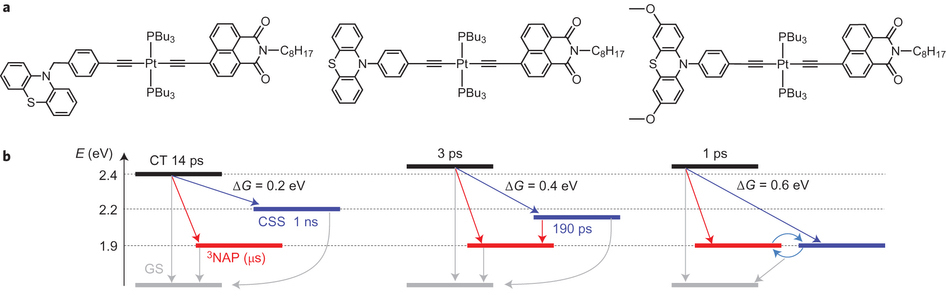
\includegraphics[width=1.7\columnwidth]{Chapters/chap4/Images/molecules.jpg}%
%   \end{adjustbox}\label{JuliaStruct}
% \end{figure}

\begin{figure*}[!t]
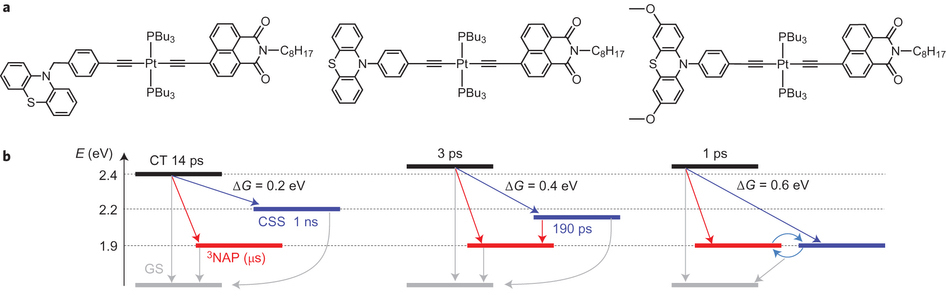
\includegraphics[width=\columnwidth]{Chapters/chap4/Images/molecules.jpg}
\caption{\textbf{a}. Molecular structure of PTZ-CH\textsubscript{2}-Pt-NAP, PTZ-Pt-NAP and OMe-PTZ-Pt-NAP, from left to right. \textbf{b}. Energy level diagrams for the ET process, with the lifetimes and the driving force ($\Delta$G) of CT $\rightarrow$ CSS transfer  indicated. Adapted with permission from Ref.~\cite{delor2015mechanism}.\label{JuliaStruct}}
\end{figure*}

\begin{figure*}[!h]
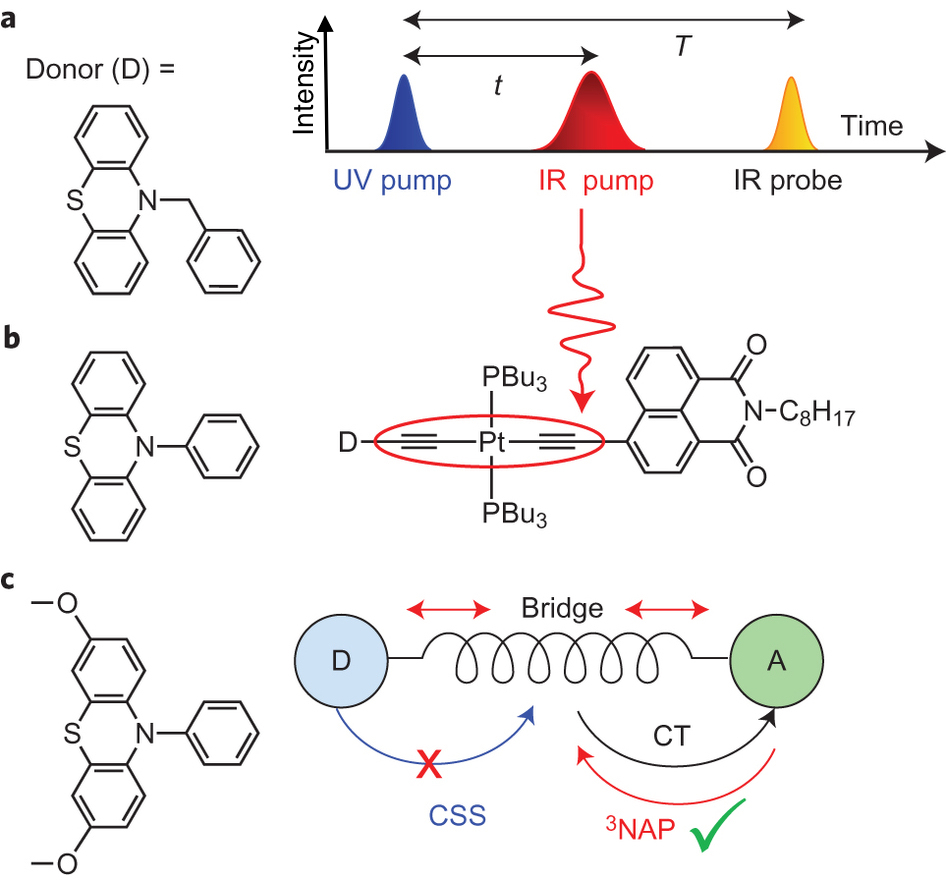
\includegraphics[width=0.71\columnwidth]{Chapters/chap4/Images/scheme.jpg}
\caption{The sketch of ET pathways. For PTZ-CH\textsubscript{2}-Pt-NAP, the CT $\rightarrow$ CSS step can be fully suppressed by intermediate infrared excitation. Reprinted with permission from Ref.~\cite{delor2015mechanism}.\label{ETscheme}}
\end{figure*}

\begin{figure*}[]
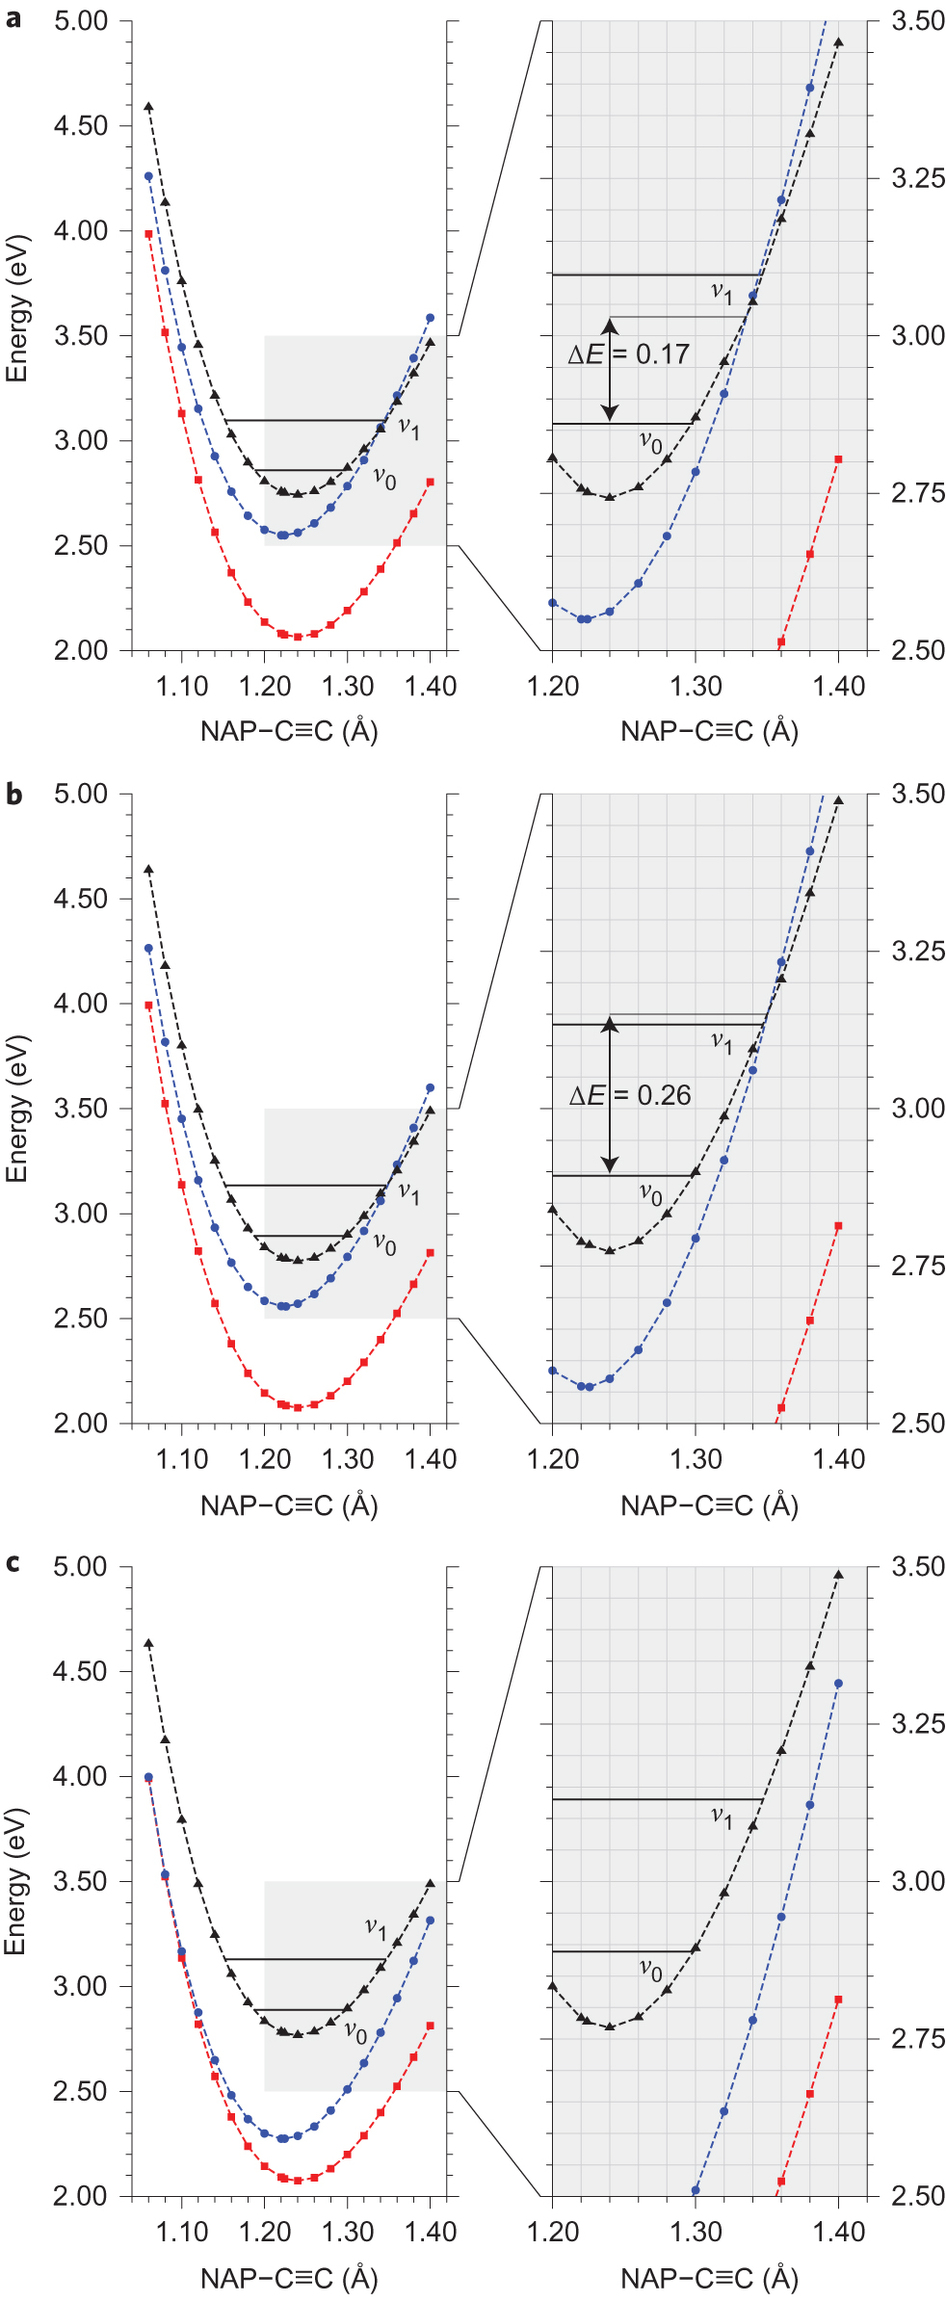
\includegraphics[width=0.44\columnwidth]{Chapters/chap4/Images/parabola.jpg}
\caption{Calculated energies of the CT (black), CSS (blue) and \textsuperscript{3}NAP (red) states along the NAP side C$\equiv$C coordinate in the ground state geometries of the molecules studied, in CH\textsubscript{2}Cl\textsubscript{2}. a, PTZ-CH\textsubscript{2}-Pt-NAP. b, PTZ-Pt-NAP. c, OMe-PTZ-Pt-NAP. The first and second vibrational energy levels for the asymmetric C$\equiv$C stretch are shown for the CT state. The energy gaps from $\nu_0$ to the intersection between CT and CSS are shown in the insets. There is a clear trend concerning the energy gap: PTZ-CH\textsubscript{2}-Pt-NAP < PTZ-Pt-NAP < OMe-PTZ-Pt-NAP, reflecting the trend experimentally observed in the efficiency of the infrared control effect. Reprinted with permission from Ref.~\cite{delor2015mechanism}.\label{PTZparabolas}} \end{figure*}


The molecules show different changes in yield because of the different donors. From PTZ-CH\textsubscript{2}-Pt-NAP to PTZ-Pt-NAP, to OMe-PTZ-Pt-NAP, the donor strength increases, which enlarges the energy gap between CT and CSS states, as sketched in Fig.~\ref{JuliaStruct}. The driving force ($\Delta$G) of CT $\rightarrow$ CSS transfer increases from 0.2 $eV$ in PTZ-CH\textsubscript{2}-Pt-NAP, to 0.4 $eV$ in PTZ-Pt-NAP, to 0.6 $eV$ in OMe-PTZ-Pt-NAP. Large $\Delta$G accelerates the CT decay and hence decreases the lifetime of CT state.
Comparing  PTZ-Pt-NAP and PTZ-CH\textsubscript{2}-Pt-NAP, CT transfer to both charge separation and recombination slows down by a factor of \textasciitilde 5 (the lifetime of CT increases from 3.3 to 14 ps and CSS from 190 ps to 1 ns). By appending methoxy groups to the PTZ, the donor strength is increased, and reaction is accelerated. As the result, the lifetime of CT in OMe-PTZ-Pt-NAP is further reduced to 1 ps.

Weinstein proposes the effect of infrared control is caused by the fact that the distance between CT energy minimum and the intersection of CT and CSS potential energy surfaces is small. For all three molecules, two PESs intersect where C$\equiv$C bond is slightly longer than the equilibrium length. When C$\equiv$C bond gets excited, it elongates and helps molecules to pass the intersection. If the energy gap between intersection and equilibrium geometry is much larger than C$\equiv$C vibrational energy, the dynamics is barely affected; if the energy gap is small, the vibrational excitation can radically change the dynamics.
% It agrees to that PTZ-CH\textsubscript{2}-Pt-NAP has the smallest energy gap in theoretical calculations, as illustrated in Fig. \ref{PTZparabolas}.
Fig. \ref{PTZparabolas} shows the calculated PESs along the NAP side C$\equiv$C coordinate in the ground state geometries. Several observations can be drawn. First, they are quite parabolic, which suggest the parabolic assumption in our approach probably holds. Second, the geometry at the intersection of CT and CSS potential energy surfaces have  longer C$\equiv$C bond than the equilibrium geometry. Third, PTZ-CH\textsubscript{2}-Pt-NAP has the smallest energy difference between the intersection and the equilibrium geometry, agreeing to the explanation above.

\section{Theoretical Model} % (fold)
% \label{sec:theoretical_model}
% The theoretical model is almost same to that presented in Section \ref{section:theory}. There is only one difference.
In previous chapters, the diabatic coupling $V_{ab}$ in Eq. \ref{mixingangle}, which determines the mixing angle $\theta$ in Eq. \ref{eq:boys}, is obtained via ER localization, while in this chapter it is computed via the generalized Mulliken-Hush (GMH) model \cite{cave1996generalization,cave1997calculation}. In principle, any diabatization approach can be used to parametrize Eq. \ref{mixingangle} There are many diabatization approaches (for a review, see Ref.~\cite{domcke2004conical}), and can be classified into three categories. ER localization and GMH approach fall in one category \cite{subotnik2008constructing,subotnik2009initial}. They do not seek diabatic states with zero derivative couplings, which are expensive to compute. Instead, they rely on physical intuition. GMH works well for linear or near-linear systems, but does not generalize to noncollinear system with more than two charge centers very well. ER localization can be seen as a extension of GMH which overcomes some drawbacks of GMH \cite{subotnik2009initial}. This time we obtain the  frequency and optimized geometry from Weinstein group. They do the computation in Gaussian 09 \cite{g09}, which does not support ER diabatization. Considering a typical calculation of such molecule takes months of CPU effort, we do not try to recompute it in Q-Chem. Instead, we turn to GMH. Fortunately, the molecule presented here is quite linear, and its charge centers are in the linear C$\equiv$C axis. As the result, GMH and ER localization approaches are expected to give similar results. The diabatic coupling given by GMH is
$$V_{ab}=\frac{\left(E_2-E_1\right) \left|\mu _{12}\right|}{\sqrt{\left(\mu _1-\mu _2\right){}^2+4 \mu _{12}^2}},$$
where $\left(E_2-E_1\right)$ is the vertical excitation energy, $\mu _1$ and $\mu _2$ are the dipole moments of corresponding adiabatic states, and $\mu _{12}$ is the transition dipole moment between two states.

The molecules were optimized using DFT for ground state and TD-DFT for excited states
% , with the B3LYP functional,
in Gaussian 09. The molecules are simplified to speed up the  computations. The P(Bu)\textsubscript{3} moieties and octyl chain of NAP are simplified to PH\textsubscript{3} and a methyl group, respectively. In all calculations, SDD pseudo potential and solvent model are used (see Appendix.~\ref{sec:T1input} for the details of parameters). The transition dipole moments and electron/hole distributions surfaces are calculated using Multiwfn 3.3.8 \cite{lu2012multiwfn}.

% section theoretical_model (end)



\section{Results and Discussion} % (fold)

\subsection{Rate Constant}
The results presented here are for PTZ-Pt-NAP. The computation of other two molecules are in progress. We optimize and get two states of PTZ-Pt-NAP, the \textsuperscript{3}NAP and the lowest CT state. The energy diagram is sketched in Fig. \ref{ene_diagram}, together with the electron/hole distribution plots. At both \textsuperscript{3}NAP or CT state geometries, the lowest state is the \textsuperscript{3}NAP, and there are two CT states above the CSS state. We can use parameters obtained at CT state geometry to compute transitions involving the CT state, and  for \textsuperscript{3}NAP involved transitions, we use  \textsuperscript{3}NAP geometry. Obviously, for the CT $\rightarrow$ \textsuperscript{3}NAP transition, we can use either geometry of CT or \textsuperscript{3}NAP.

% \begin{figure}[!ht]
%   \begin{adjustbox}{addcode={\begin{minipage}{1.5\columnwidth}}{\caption{%
%      The energy diagram of triplet states at \textsuperscript{3}NAP and CT state geometries. The electron/hole distribution are shown as well (green for electron, blue for hole). The arrows indicate the transitions we calculate.
%       }\end{minipage}},rotate=90,center}
%       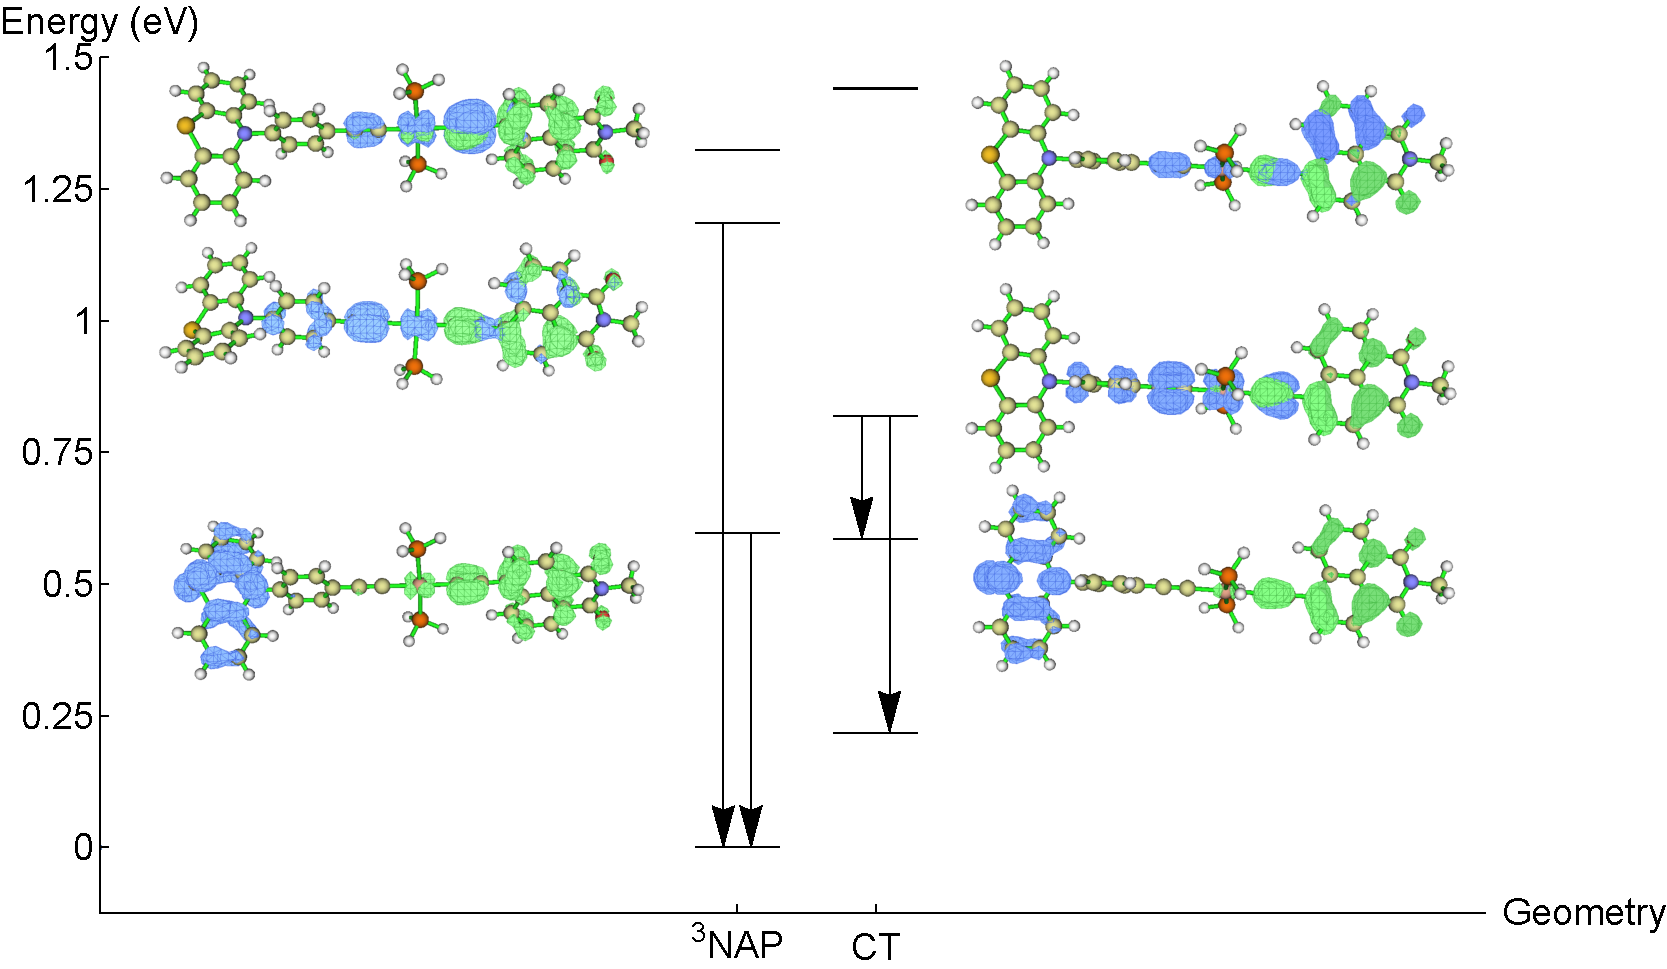
\includegraphics[width=2\columnwidth]{Chapters/chap4/Images/energy_diagram.pdf}%
%   \end{adjustbox}
% \end{figure}

\begin{figure}[]
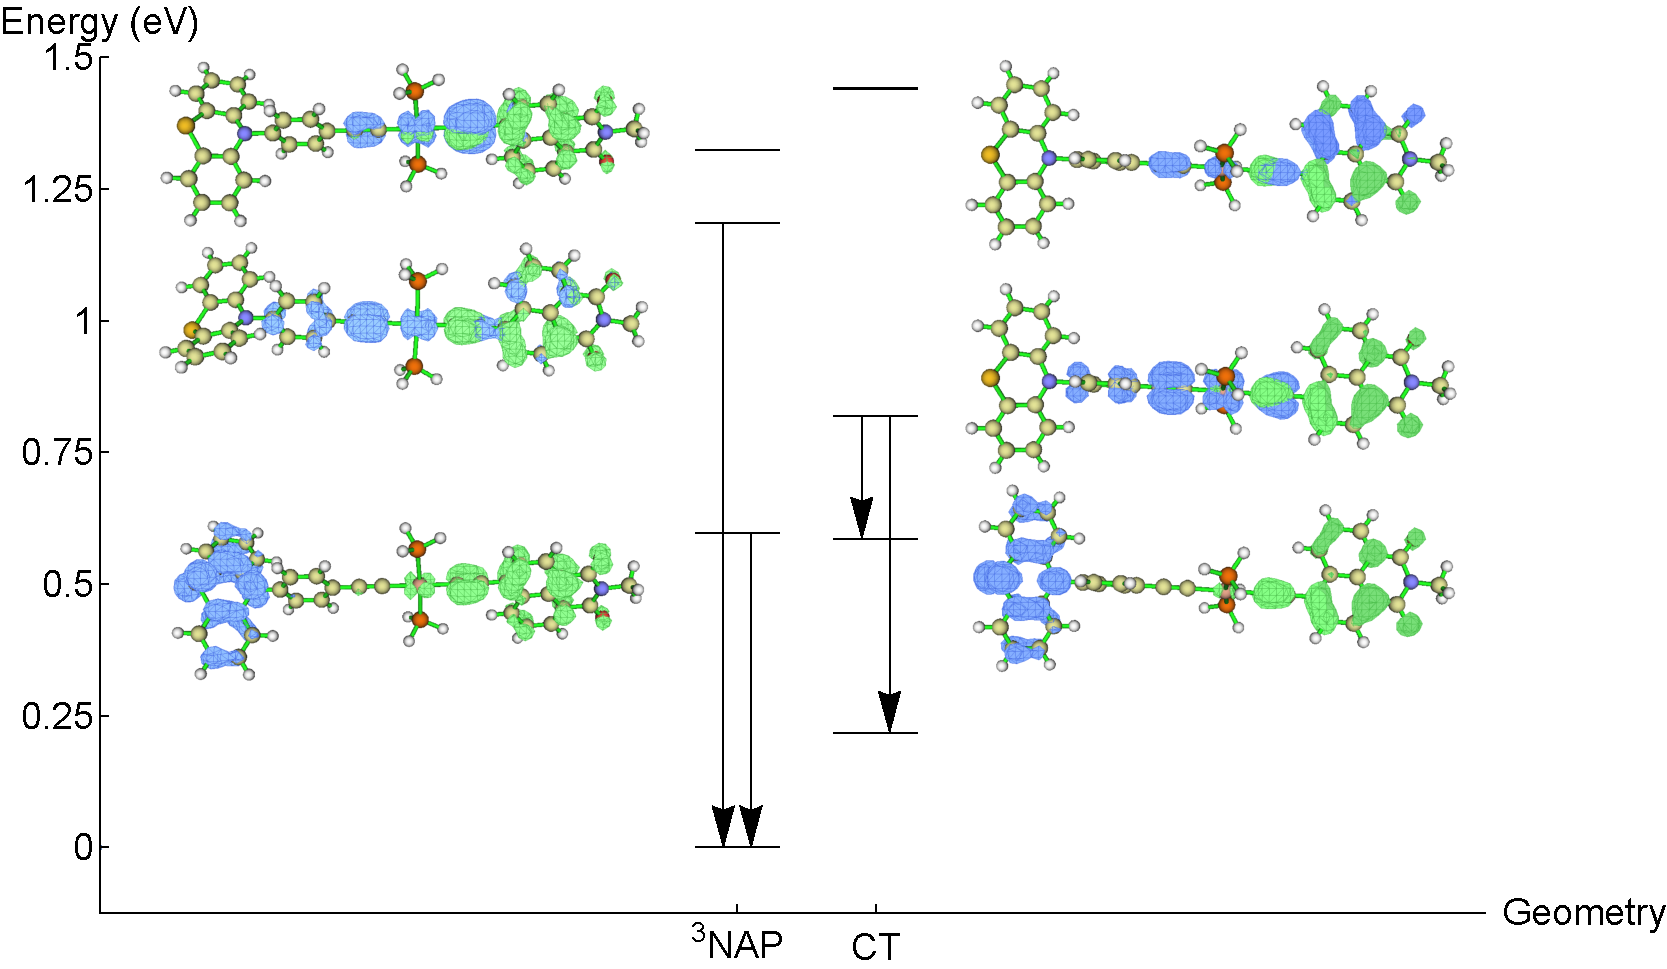
\includegraphics[width=\columnwidth]{Chapters/chap4/Images/energy_diagram.pdf}
\caption{The energy diagram of triplet states at \textsuperscript{3}NAP and CT state geometries. The electron/hole distribution are shown as well (green for electron, blue for hole). The arrows indicate the transitions we calculate.
}\label{ene_diagram}
\end{figure}


The comparison between theoretical and experimental rate constants is summarized in Fig. \ref{rateComp}. We calculate several sets of theoretical rates. First, we calculate the Marcus theory rates (Eq. \ref{eq:marcus}). At the CT geometry, we get good agreement. However, at the \textsuperscript{3}NAP geometry, the results are very poor. Second, we calculate the TCLME rates (Eq. \ref{gr-expression}). The results are still not satisfactory for the \textsuperscript{3}NAP geometry. Nevertheless, TCLME is better than Marcus theory in all cases. We also calculate the TCLME rates with only the primary mode used. Still, they agree to the exact TCLME rates better at the CT geometry.

The failure of the \textsuperscript{3}NAP geometry is especially obvious when we look at the CT $\rightarrow$ \textsuperscript{3}NAP transition. For this transition, we can calculate at either geometry. The TCLME rate constants at two geometries do not agree to each other. The results based on the CT geometry are in the same magnitude with experimental values, and the corresponding primary mode rates are similar to the exact ones. While the \textsuperscript{3}NAP geometry performs poorly. In Section \ref{sec:condon}, we illustrate that the error is, at least partially, caused by the break down of Condon approximation, and according corrections may improve the results.

\begin{figure*}[]
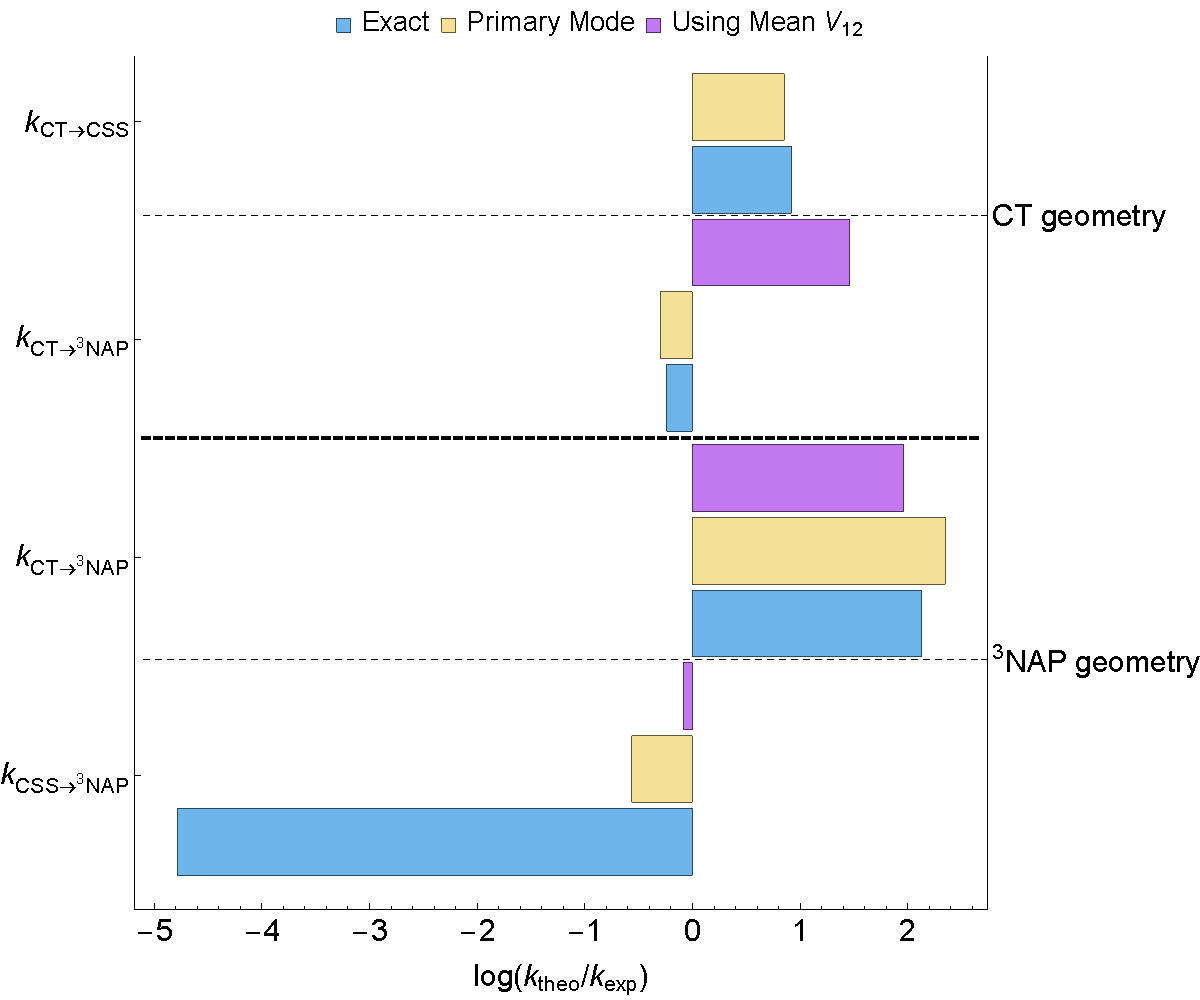
\includegraphics[width=\columnwidth]{Chapters/chap4/Images/kTCLME-VS-EXPT.pdf}
\caption{Comparisons between theoretical rate constants and the experimental rates. Experimental rates are calculated as yield of product/lifetime of reactant, using values from ~Ref. \cite{delor2015mechanism}.  The ``Marcus'' rates are calculated using Marcus theory with the diabatic couplings at according geometries. The ``Marcus (mean V)'' rates are calculated using mean diabatic couplings along the interpolated coordinate in Fig. \ref{interCondon}. Similarly, the ``TCLME'' and ``TCLME (mean V)'' rates are calculated using the TCLME approach, with all normal modes used. The ``PLM'' rates are calculated using only the primary mode. Our approach performs better than Marcus theory. The CT geometry gives good ``exact'' results, its primary mode rates also agree well. While for the \textsuperscript{3}NAP geometry, using mean value of diabatic couplings along the reaction coordinate significantly improves the performance.\label{rateComp}}
\end{figure*}



\begin{figure}[]
\subfloat[]{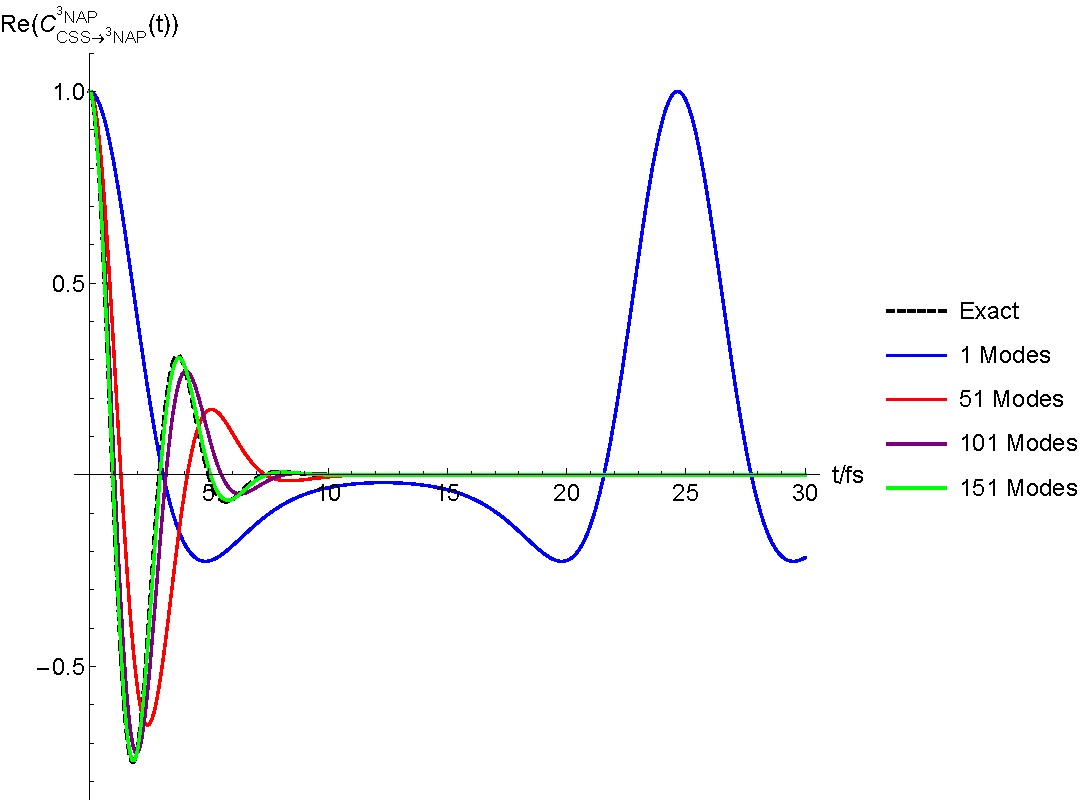
\includegraphics[width=0.5\columnwidth]{Chapters/chap4/Images/corrT12.pdf}}
\subfloat[]{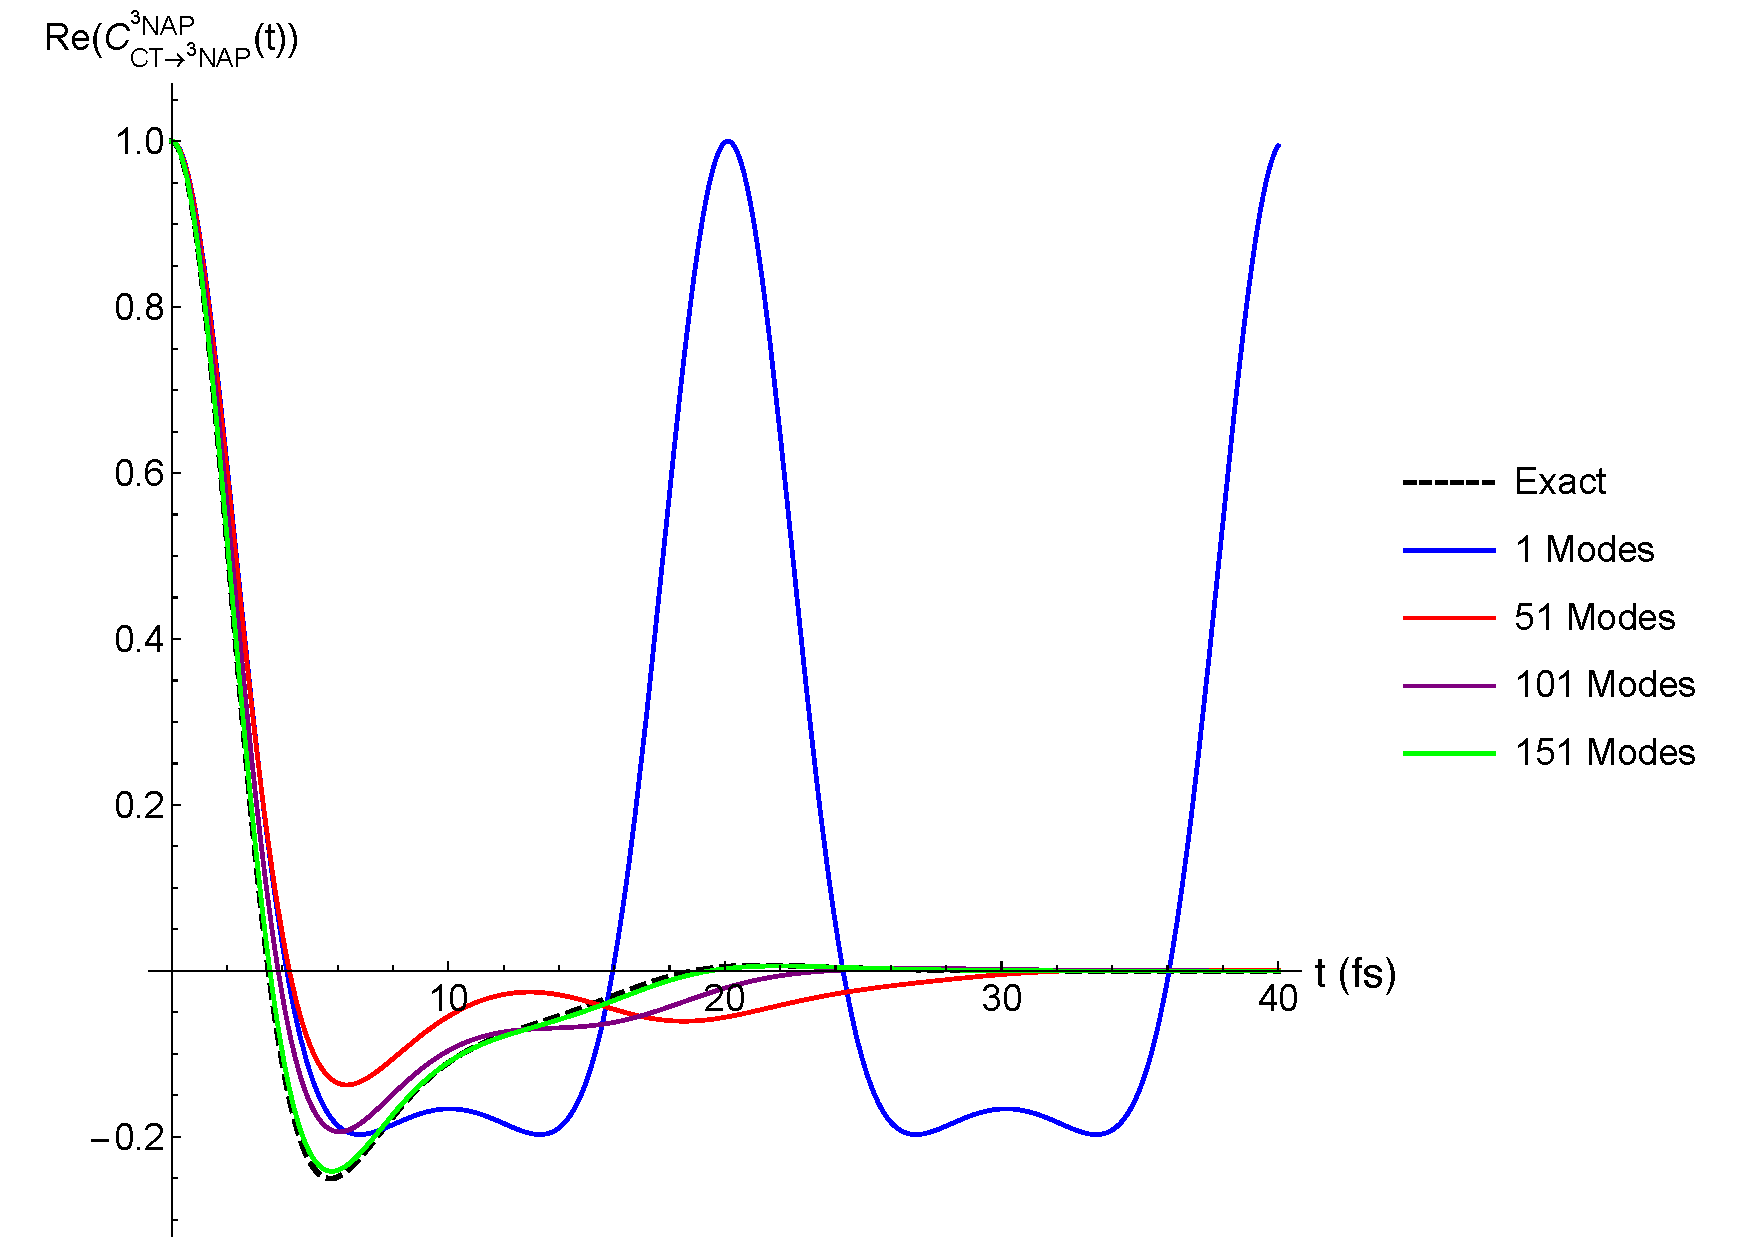
\includegraphics[width=0.5\columnwidth]{Chapters/chap4/Images/corrT13.pdf}}\\
\subfloat[]{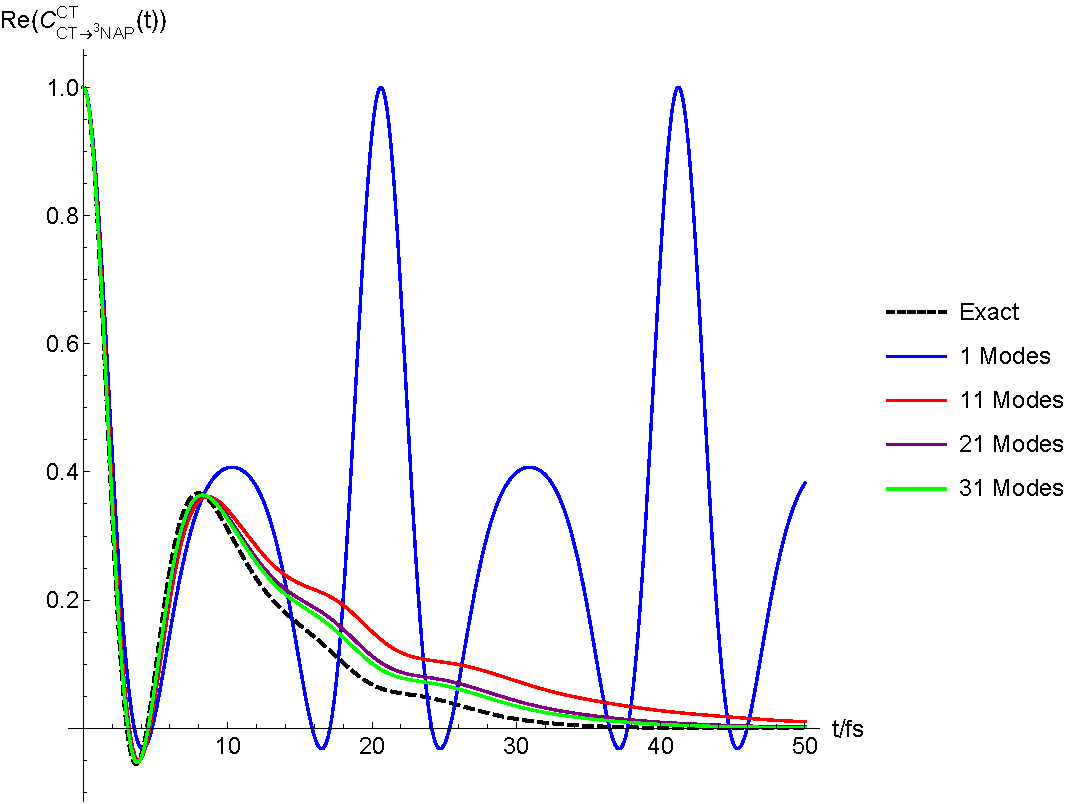
\includegraphics[width=0.5\columnwidth]{Chapters/chap4/Images/corrT31.pdf}}
\subfloat[]{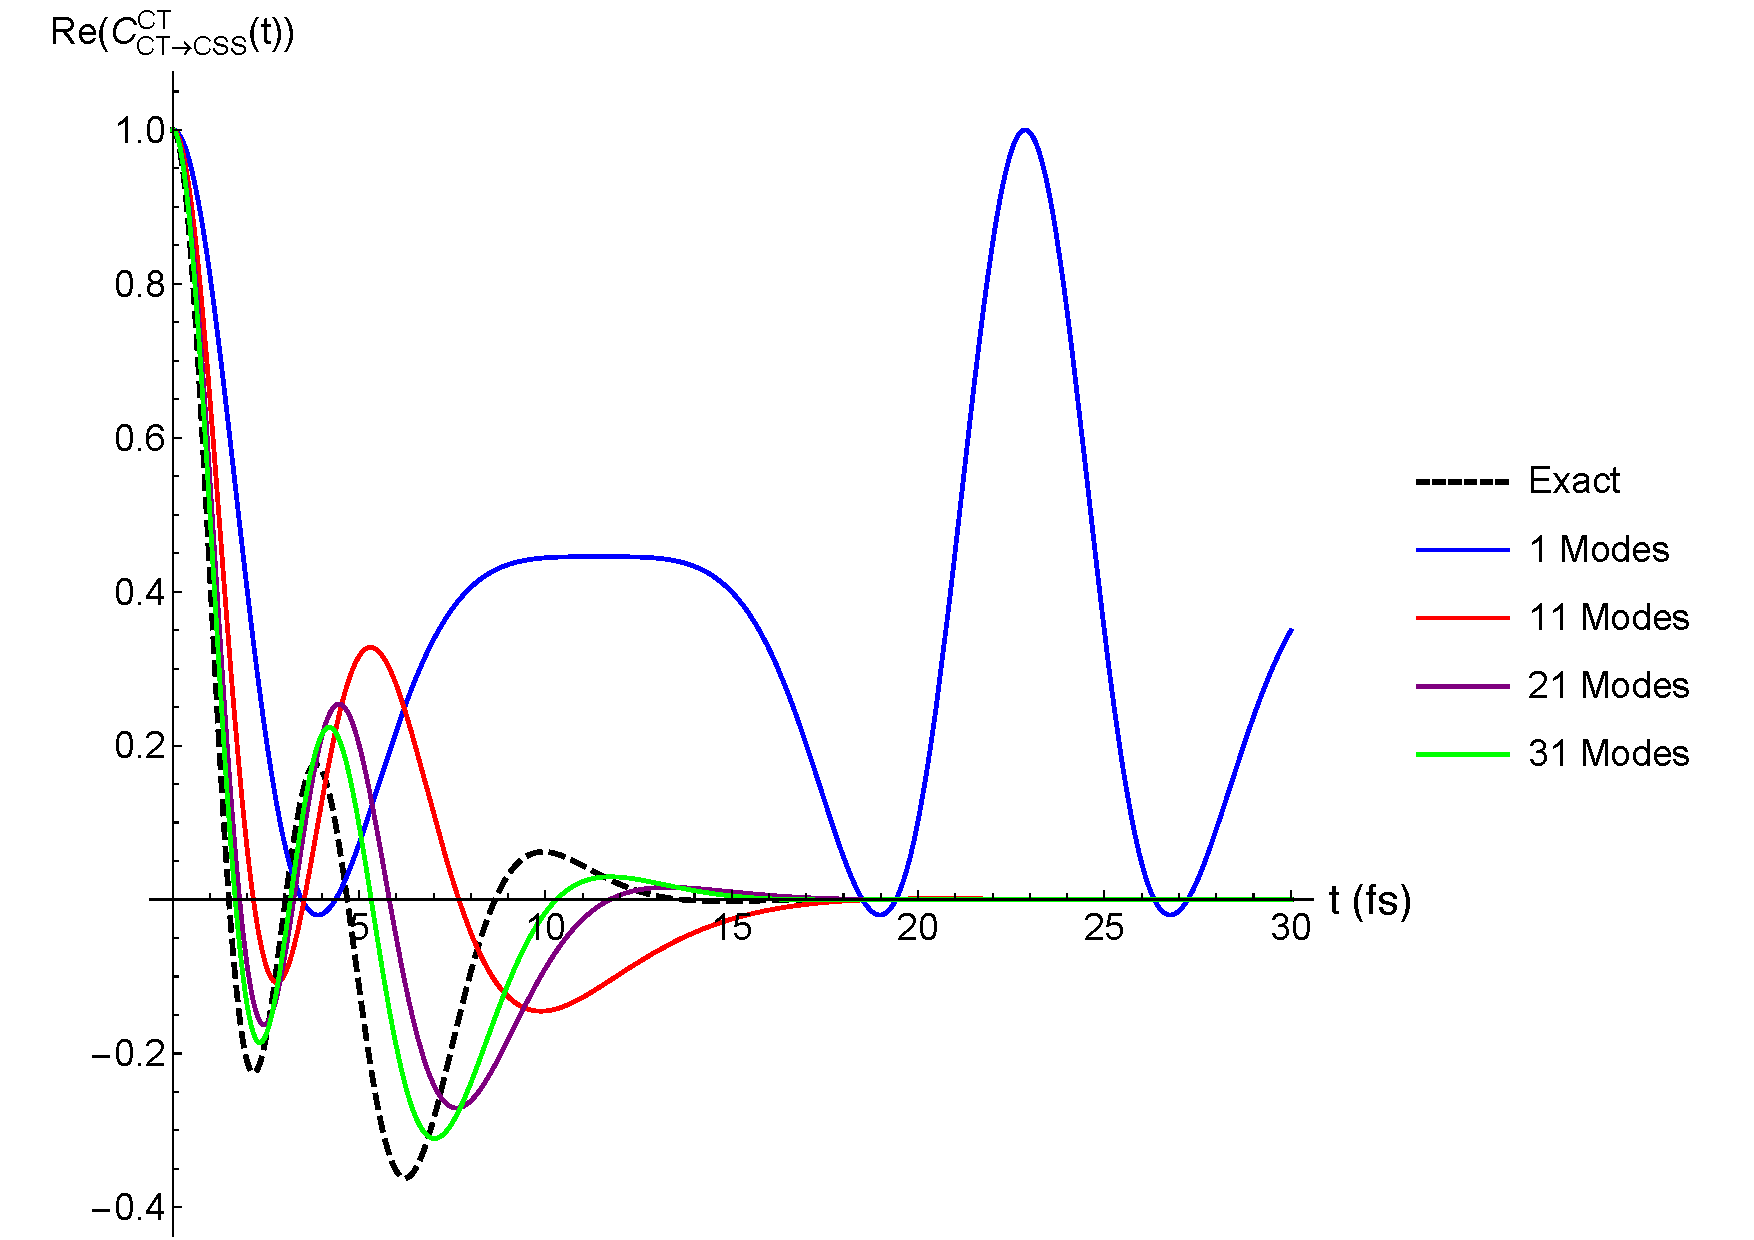
\includegraphics[width=0.5\columnwidth]{Chapters/chap4/Images/corrT32.pdf}}
\caption{
Correlation functions of various numbers of projected modes, compared to exact correlation, for (a) CSS $\rightarrow$ \textsuperscript{3}NAP at \textsuperscript{3}NAP geometry, (b) CT $\rightarrow$ \textsuperscript{3}NAP at \textsuperscript{3}NAP geometry, (c) CT $\rightarrow$ \textsuperscript{3}NAP at CT geometry, and (d) CT $\rightarrow$ CSS at CT geometry.
}\label{corrT1T3}
\end{figure}



\subsection{Primary Mode}

In Fig. \ref{rateComp} we see that for the CT geometry, using only the primary mode is sufficient to get good rate constants. Fig. \ref{corrT1T3} shows the correlation functions of different numbers of projected modes for all four transitions. Again the CT geometry performs better. Its convergence is satisfactory. The primary mode always resembles the exact initial dynamics, especially for the CT $\rightarrow$ \textsuperscript{3}NAP transition, where the primary mode reproduces the dynamics almost exactly up to 9 fs. Though not perfectly, tens of projected modes are enough to reproduce the shape of exact correlation functions for CT geometry. On the contrary, it takes hundreds of modes to recover the correlation for \textsuperscript{3}NAP (note that the degrees of freedom of PTZ-Pt-NAP is 201). Our previous studies \cite{yang2014intramolecular} shows that perfect matching of correlation function is unnecessary for good rate constant. It is verified again here. The primary mode's correlation function at CT geometry does not match the exact correlation perfectly, but the rate it gives agrees well to the exact value, and experiments. Nevertheless, the better it resembles the shape of exact function, the better the rate constant it gives.


\begin{figure}[]
\subfloat[]{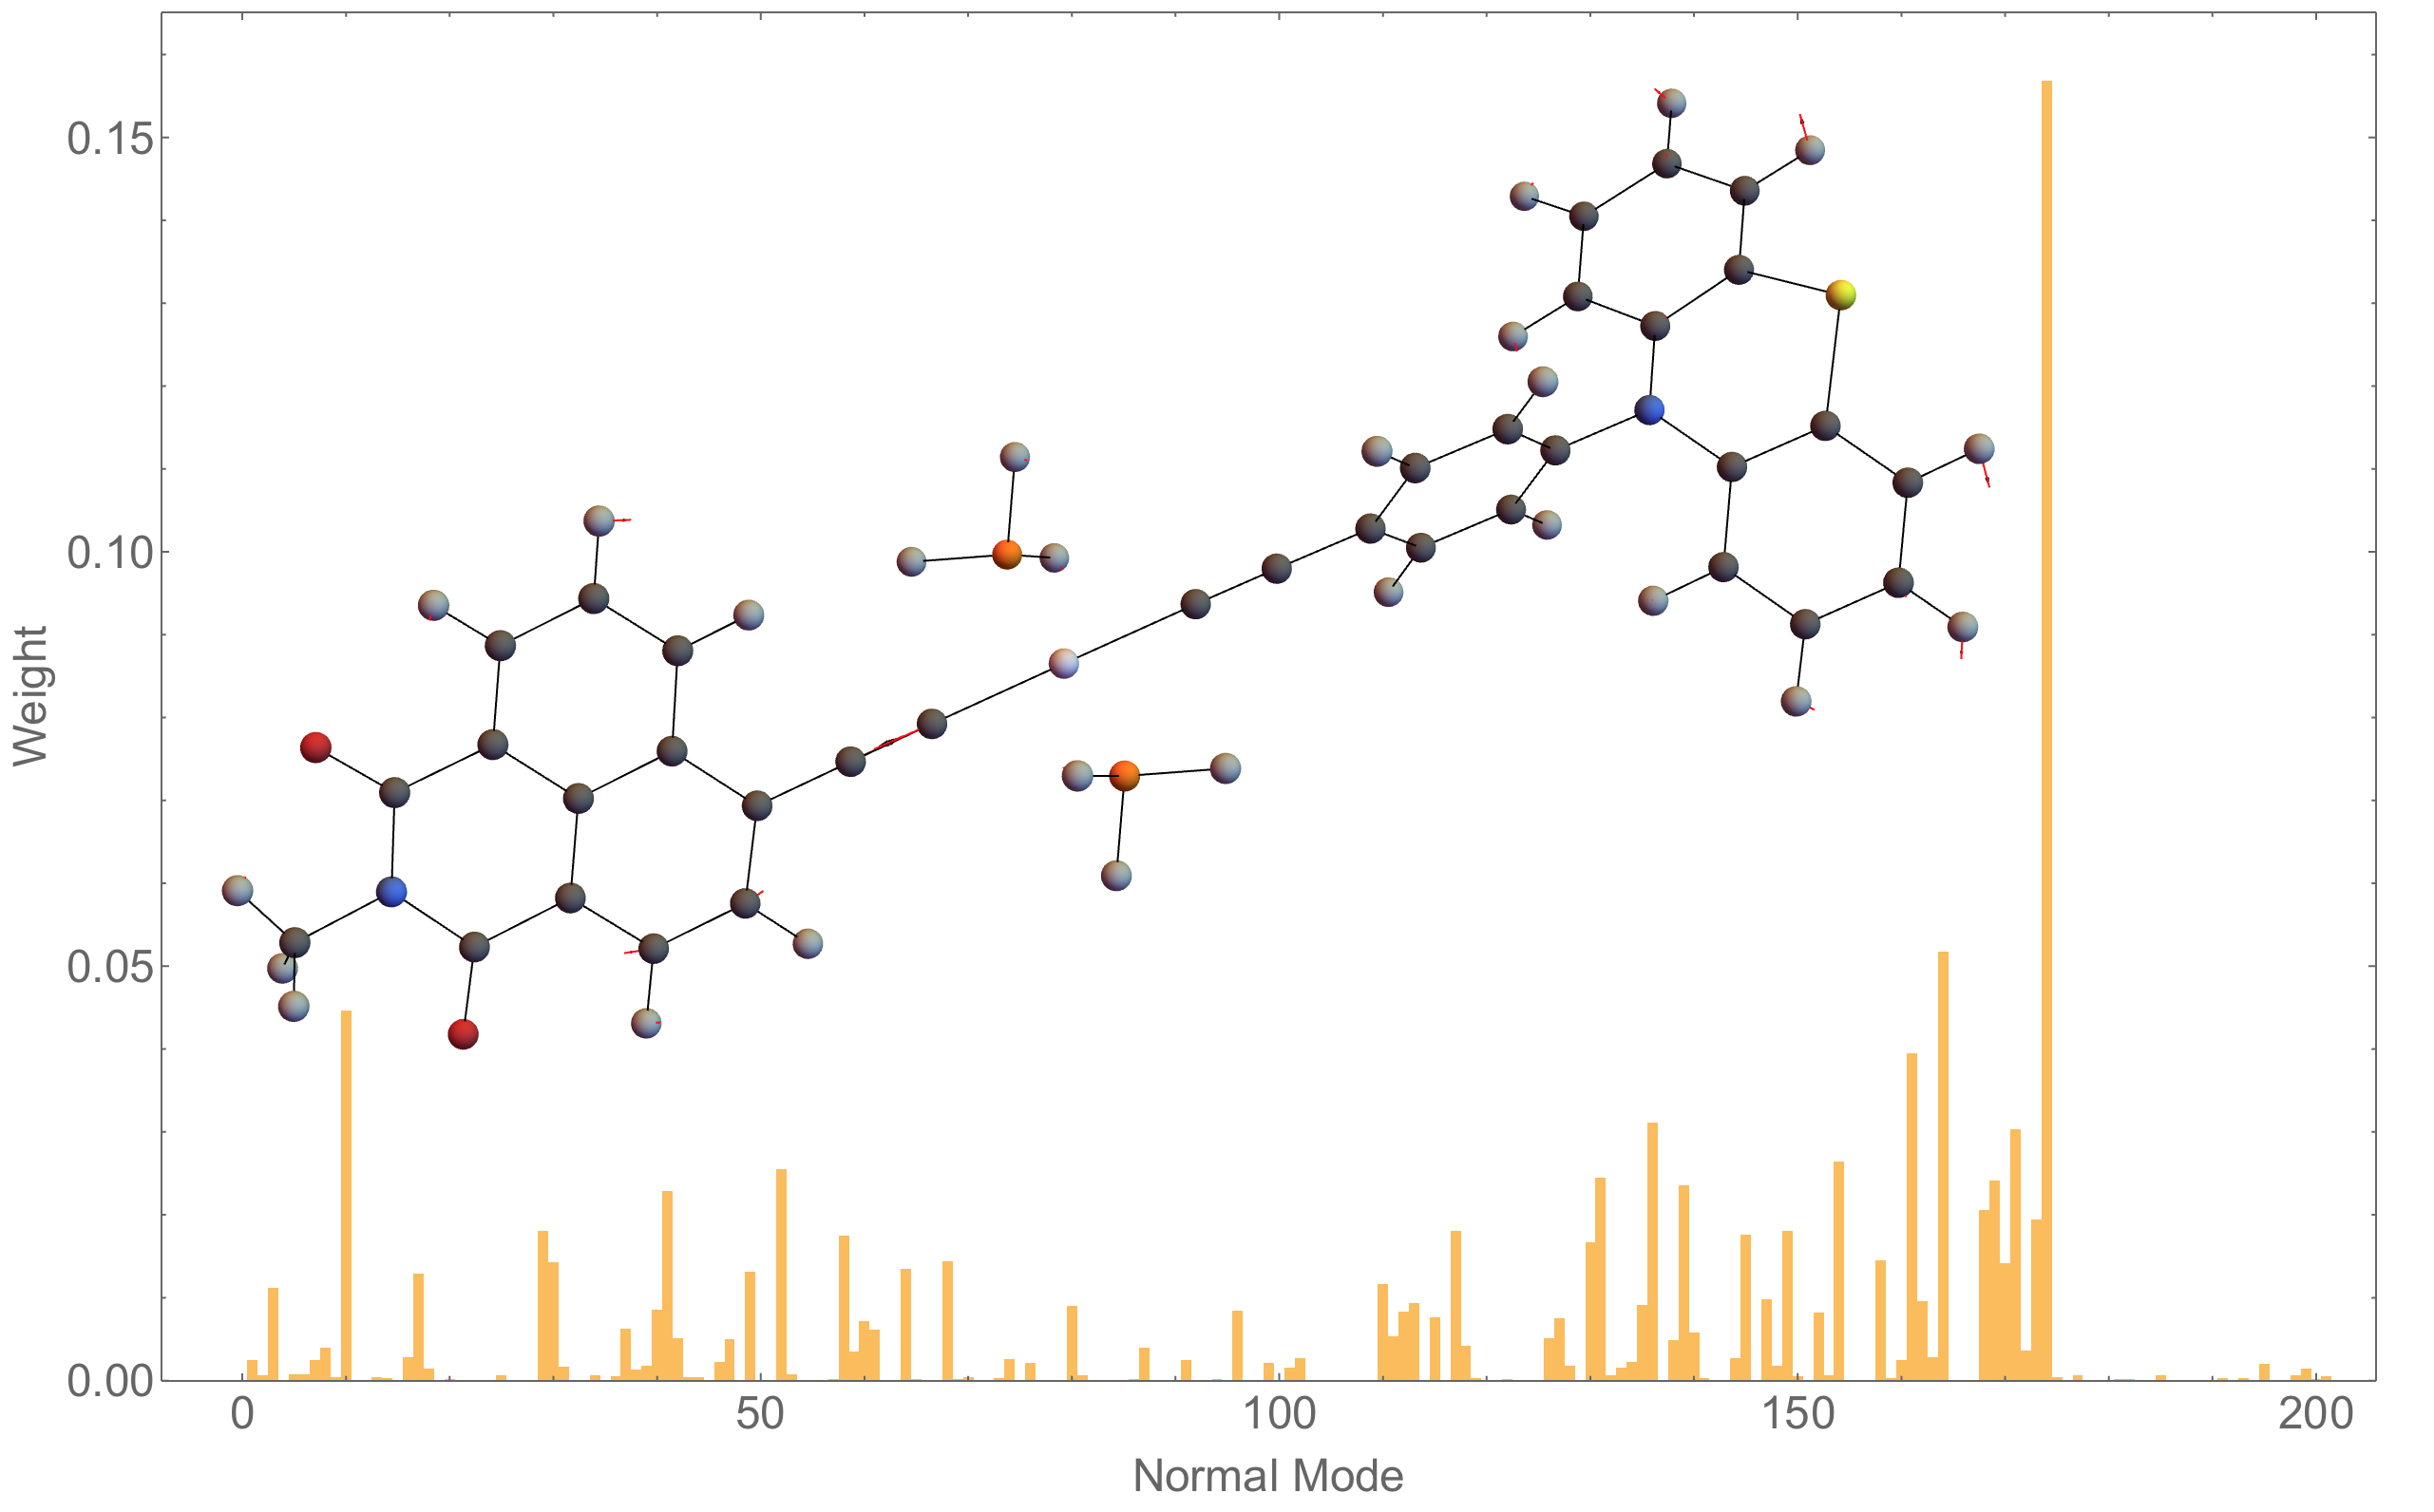
\includegraphics[width=0.84\columnwidth]{Chapters/chap4/Images/plmT12.png}}\\
\subfloat[]{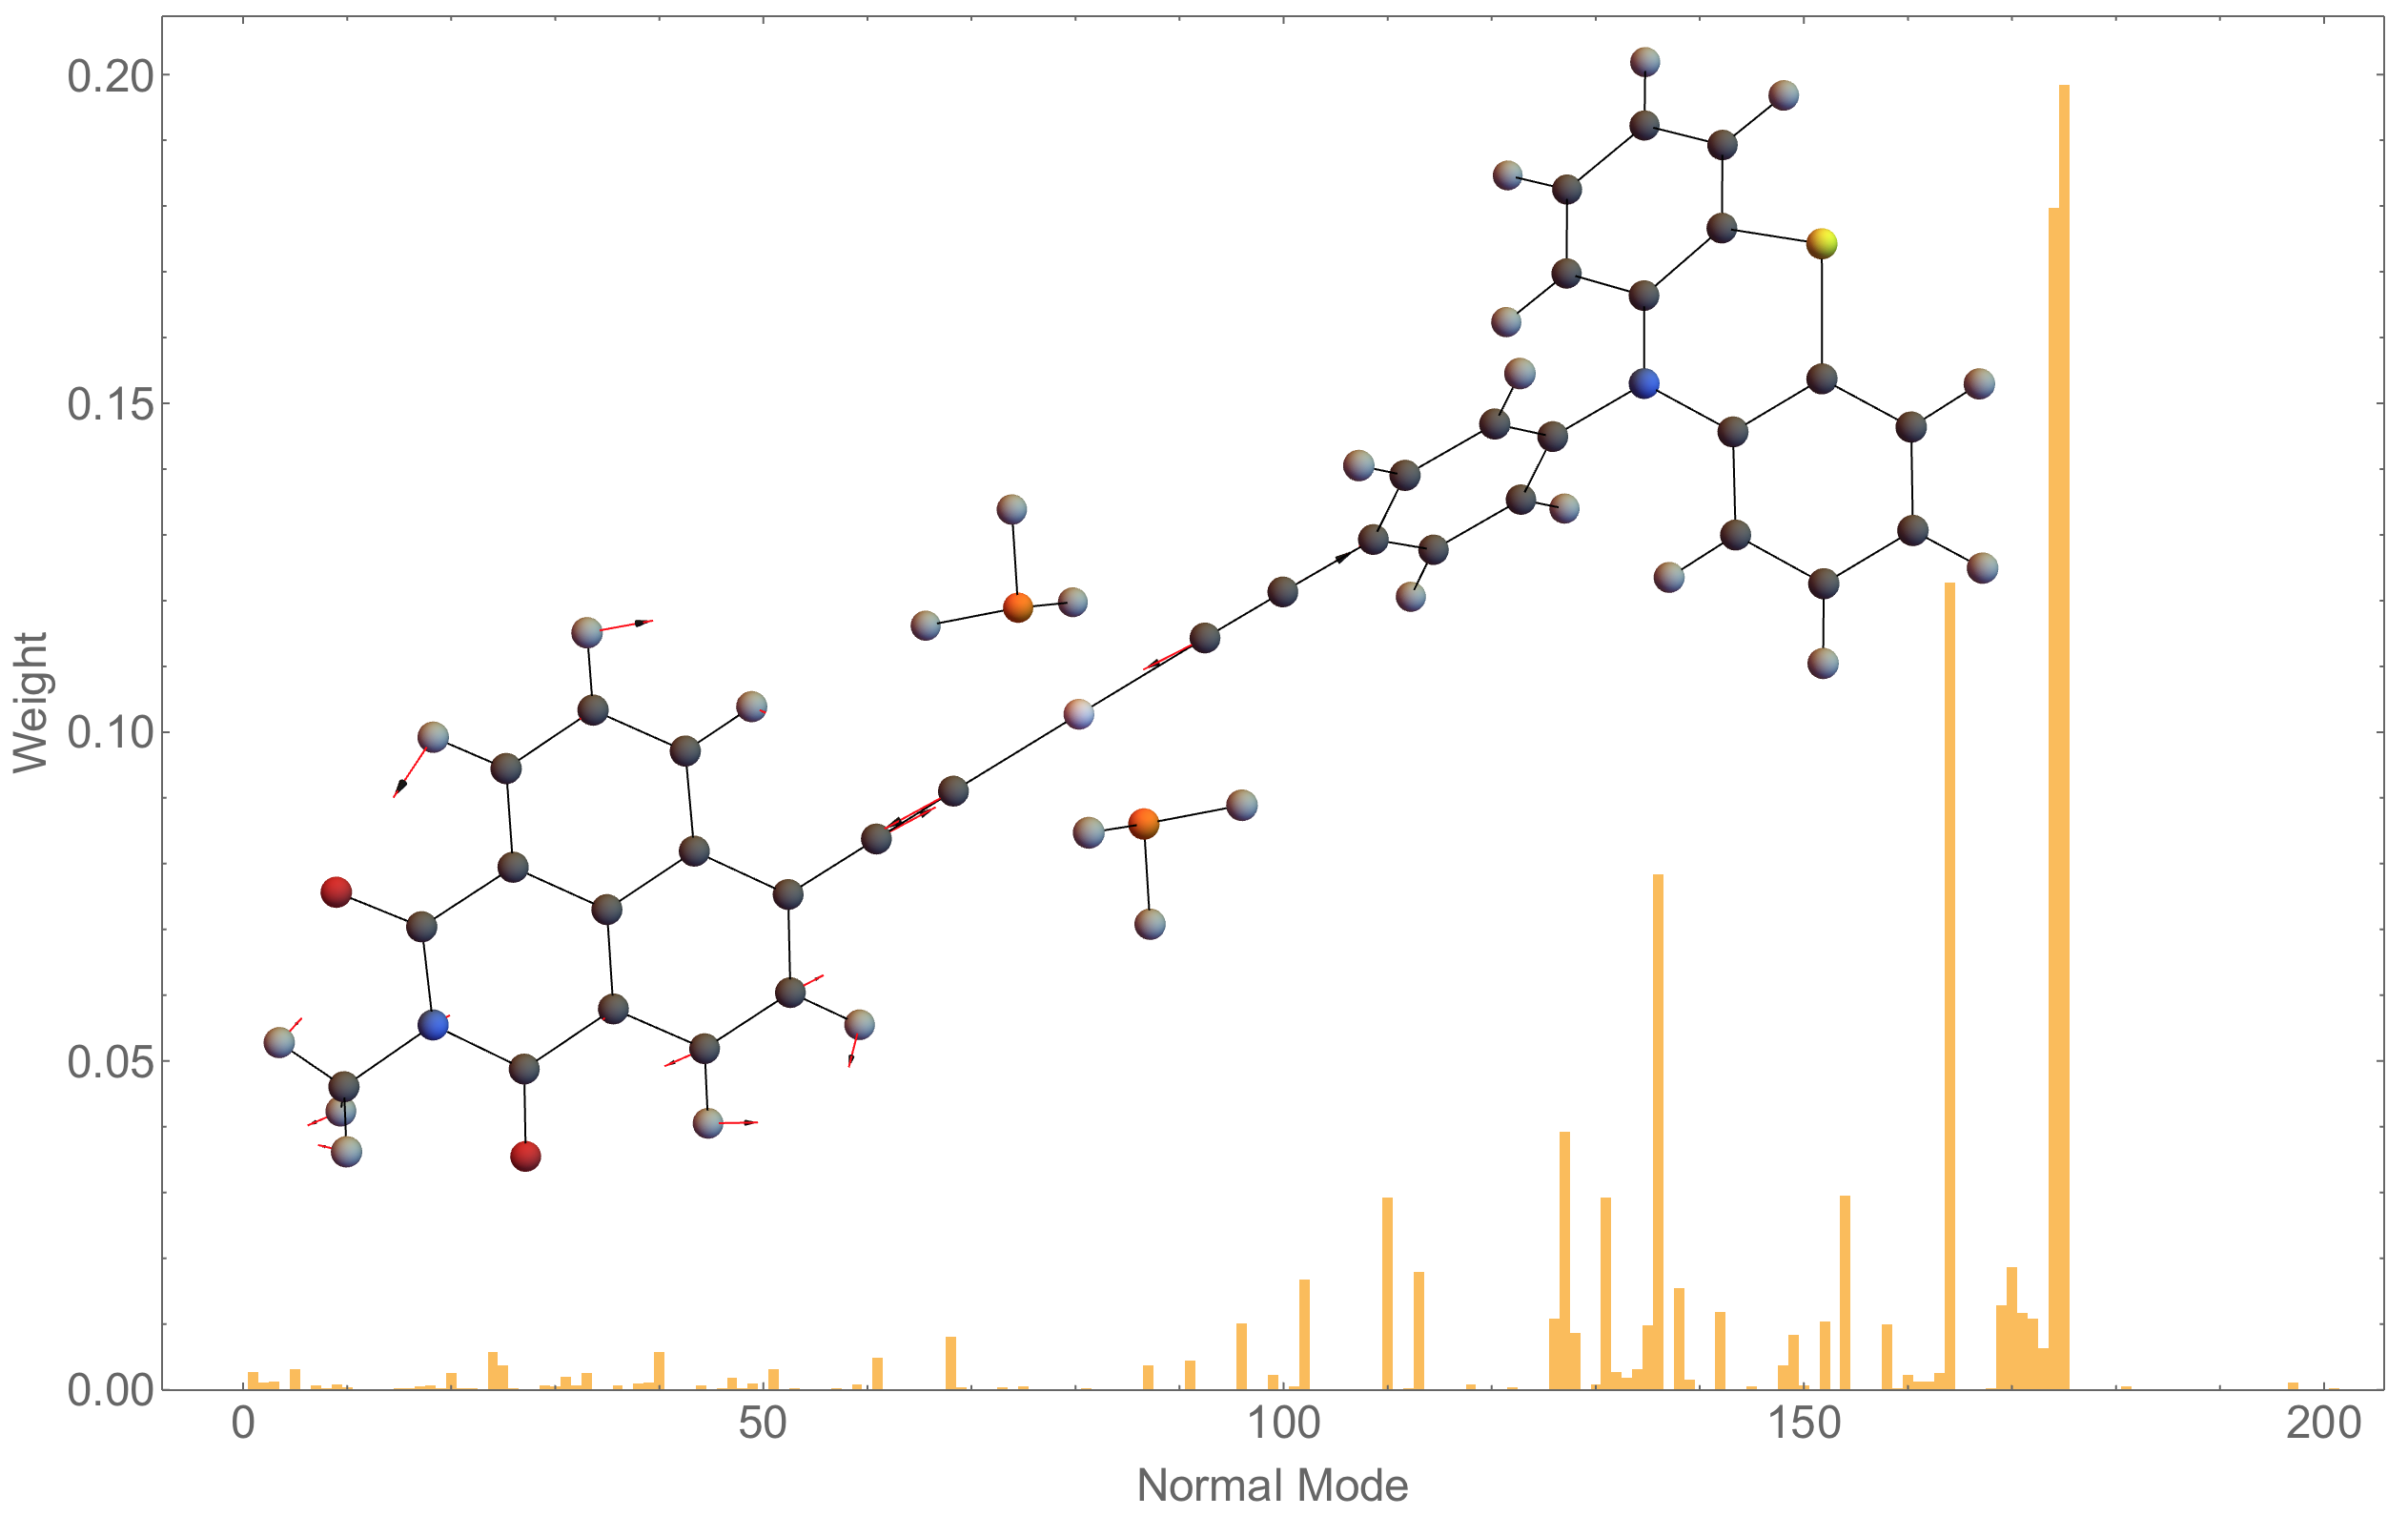
\includegraphics[width=0.84\columnwidth]{Chapters/chap4/Images/plmT13.png}}
% \subfloat[]{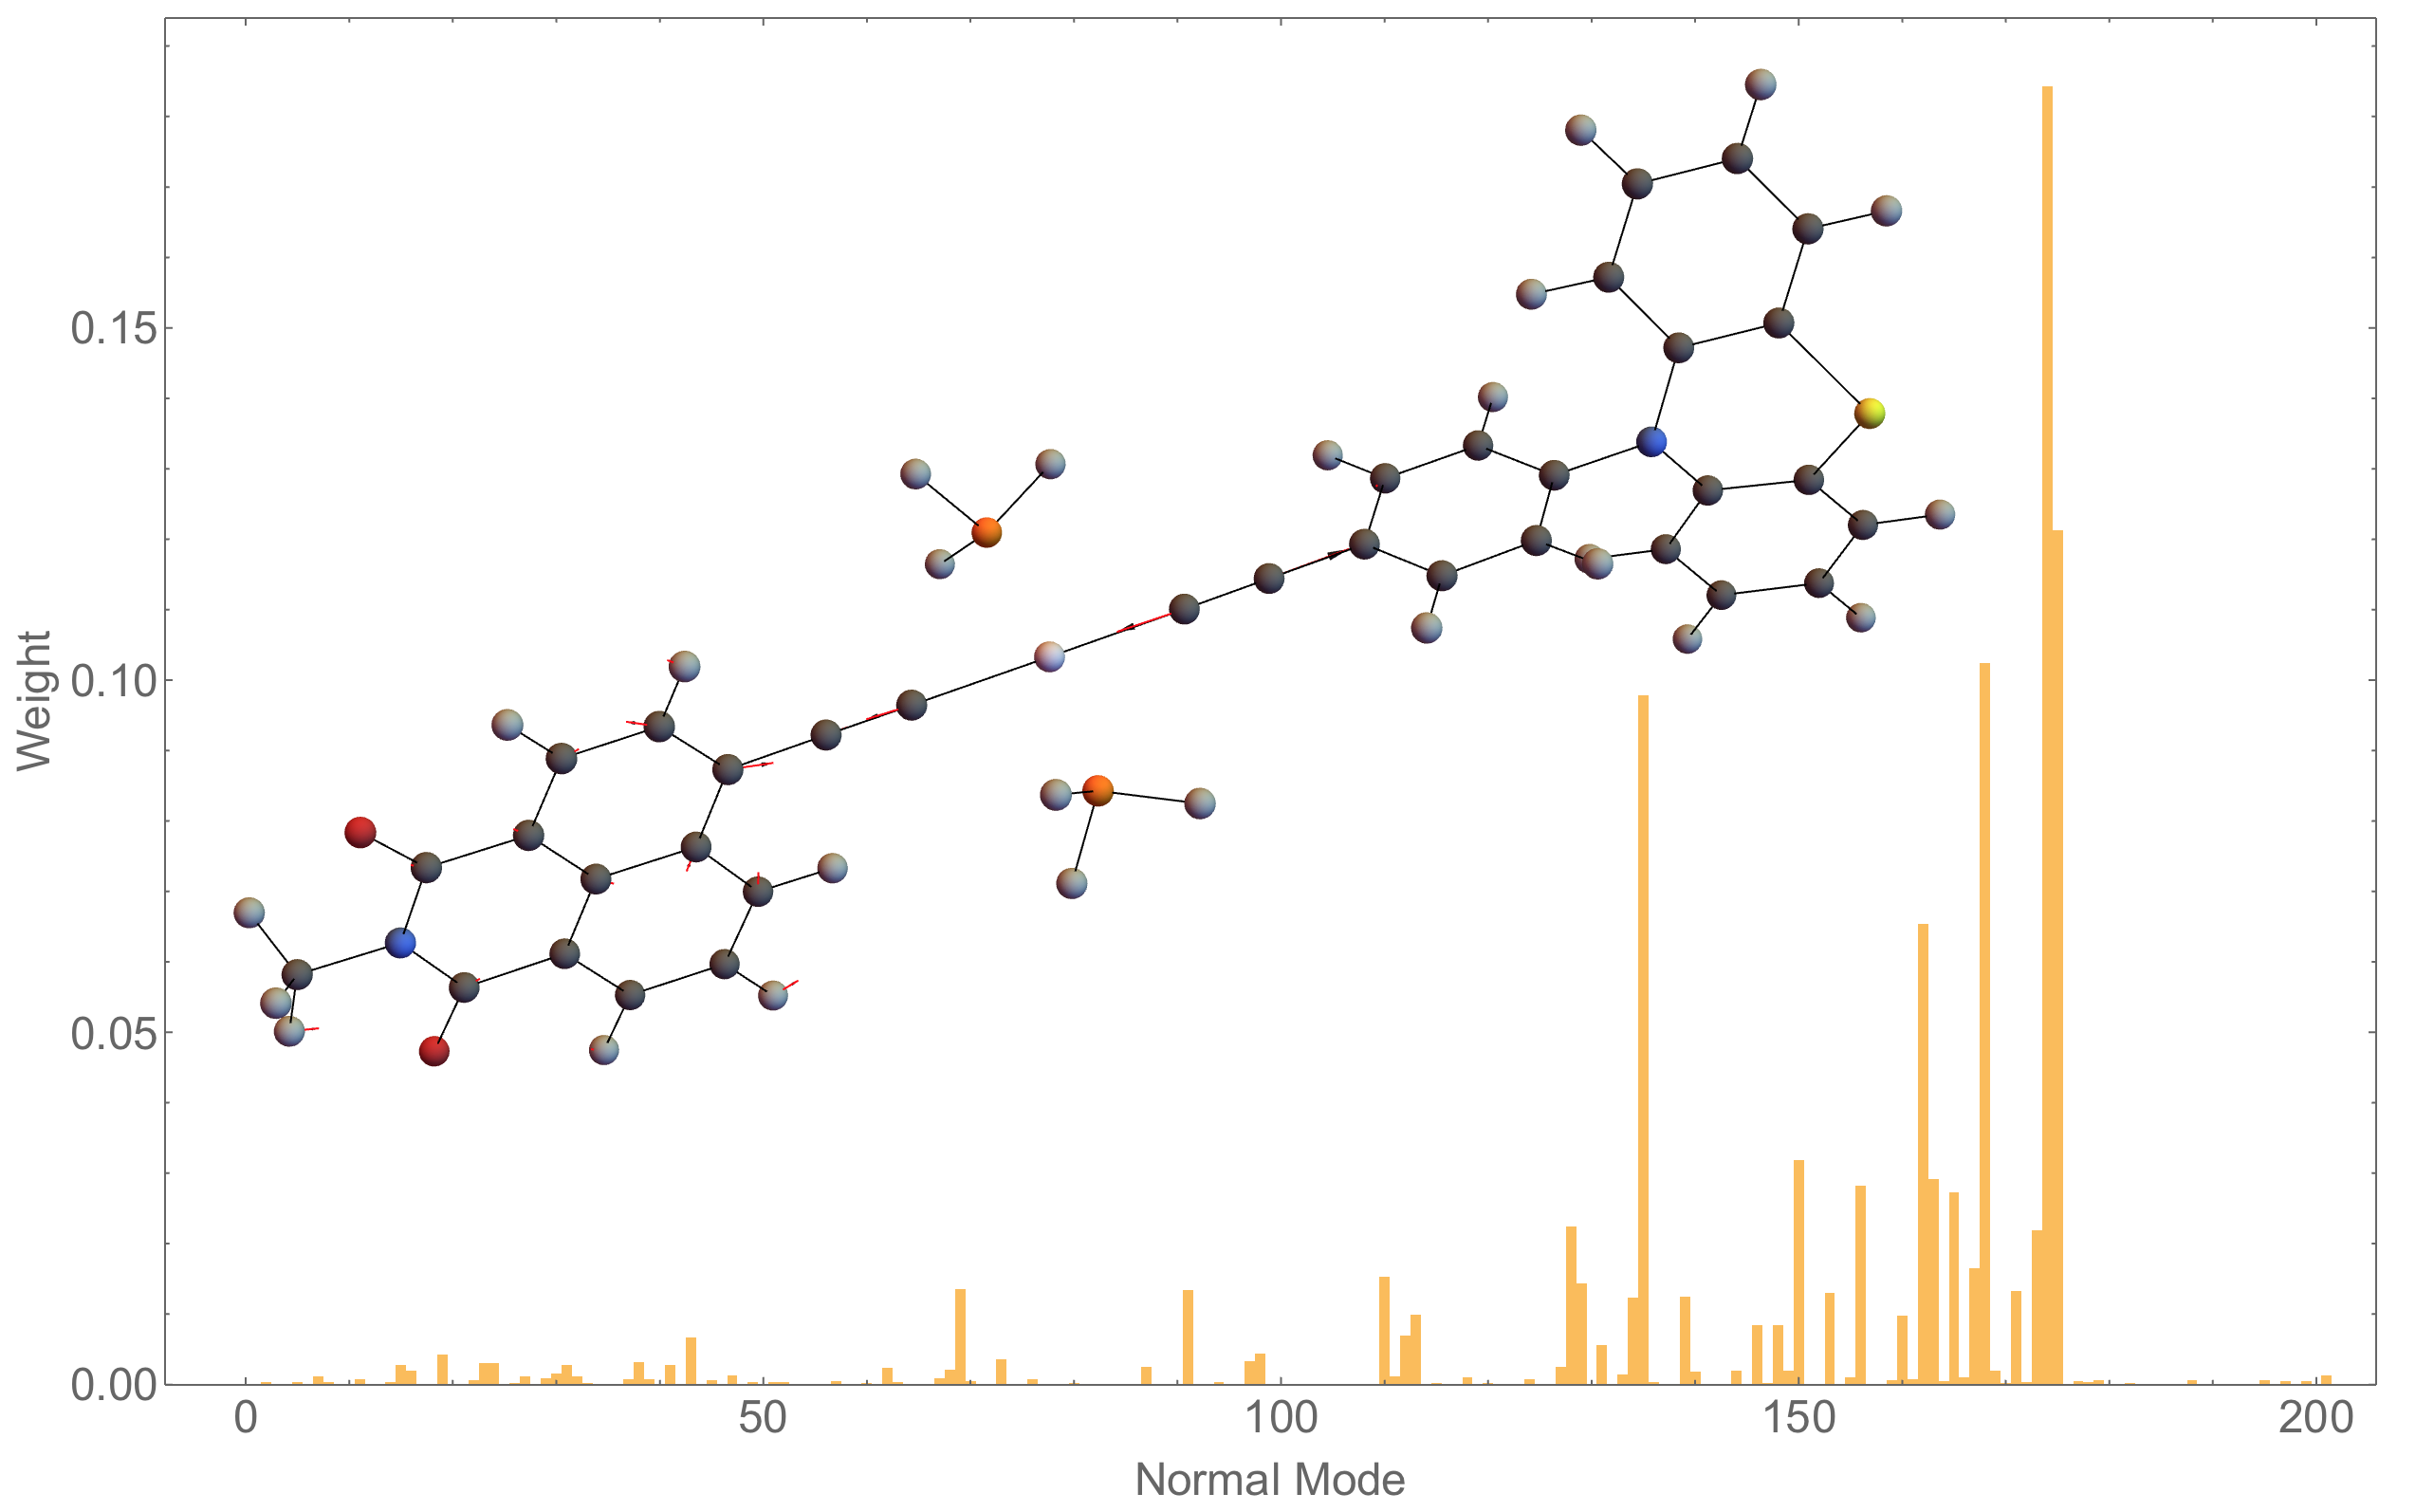
\includegraphics[width=0.88\columnwidth]{Chapters/chap4/Images/plmT31.png}}\\
% \subfloat[]{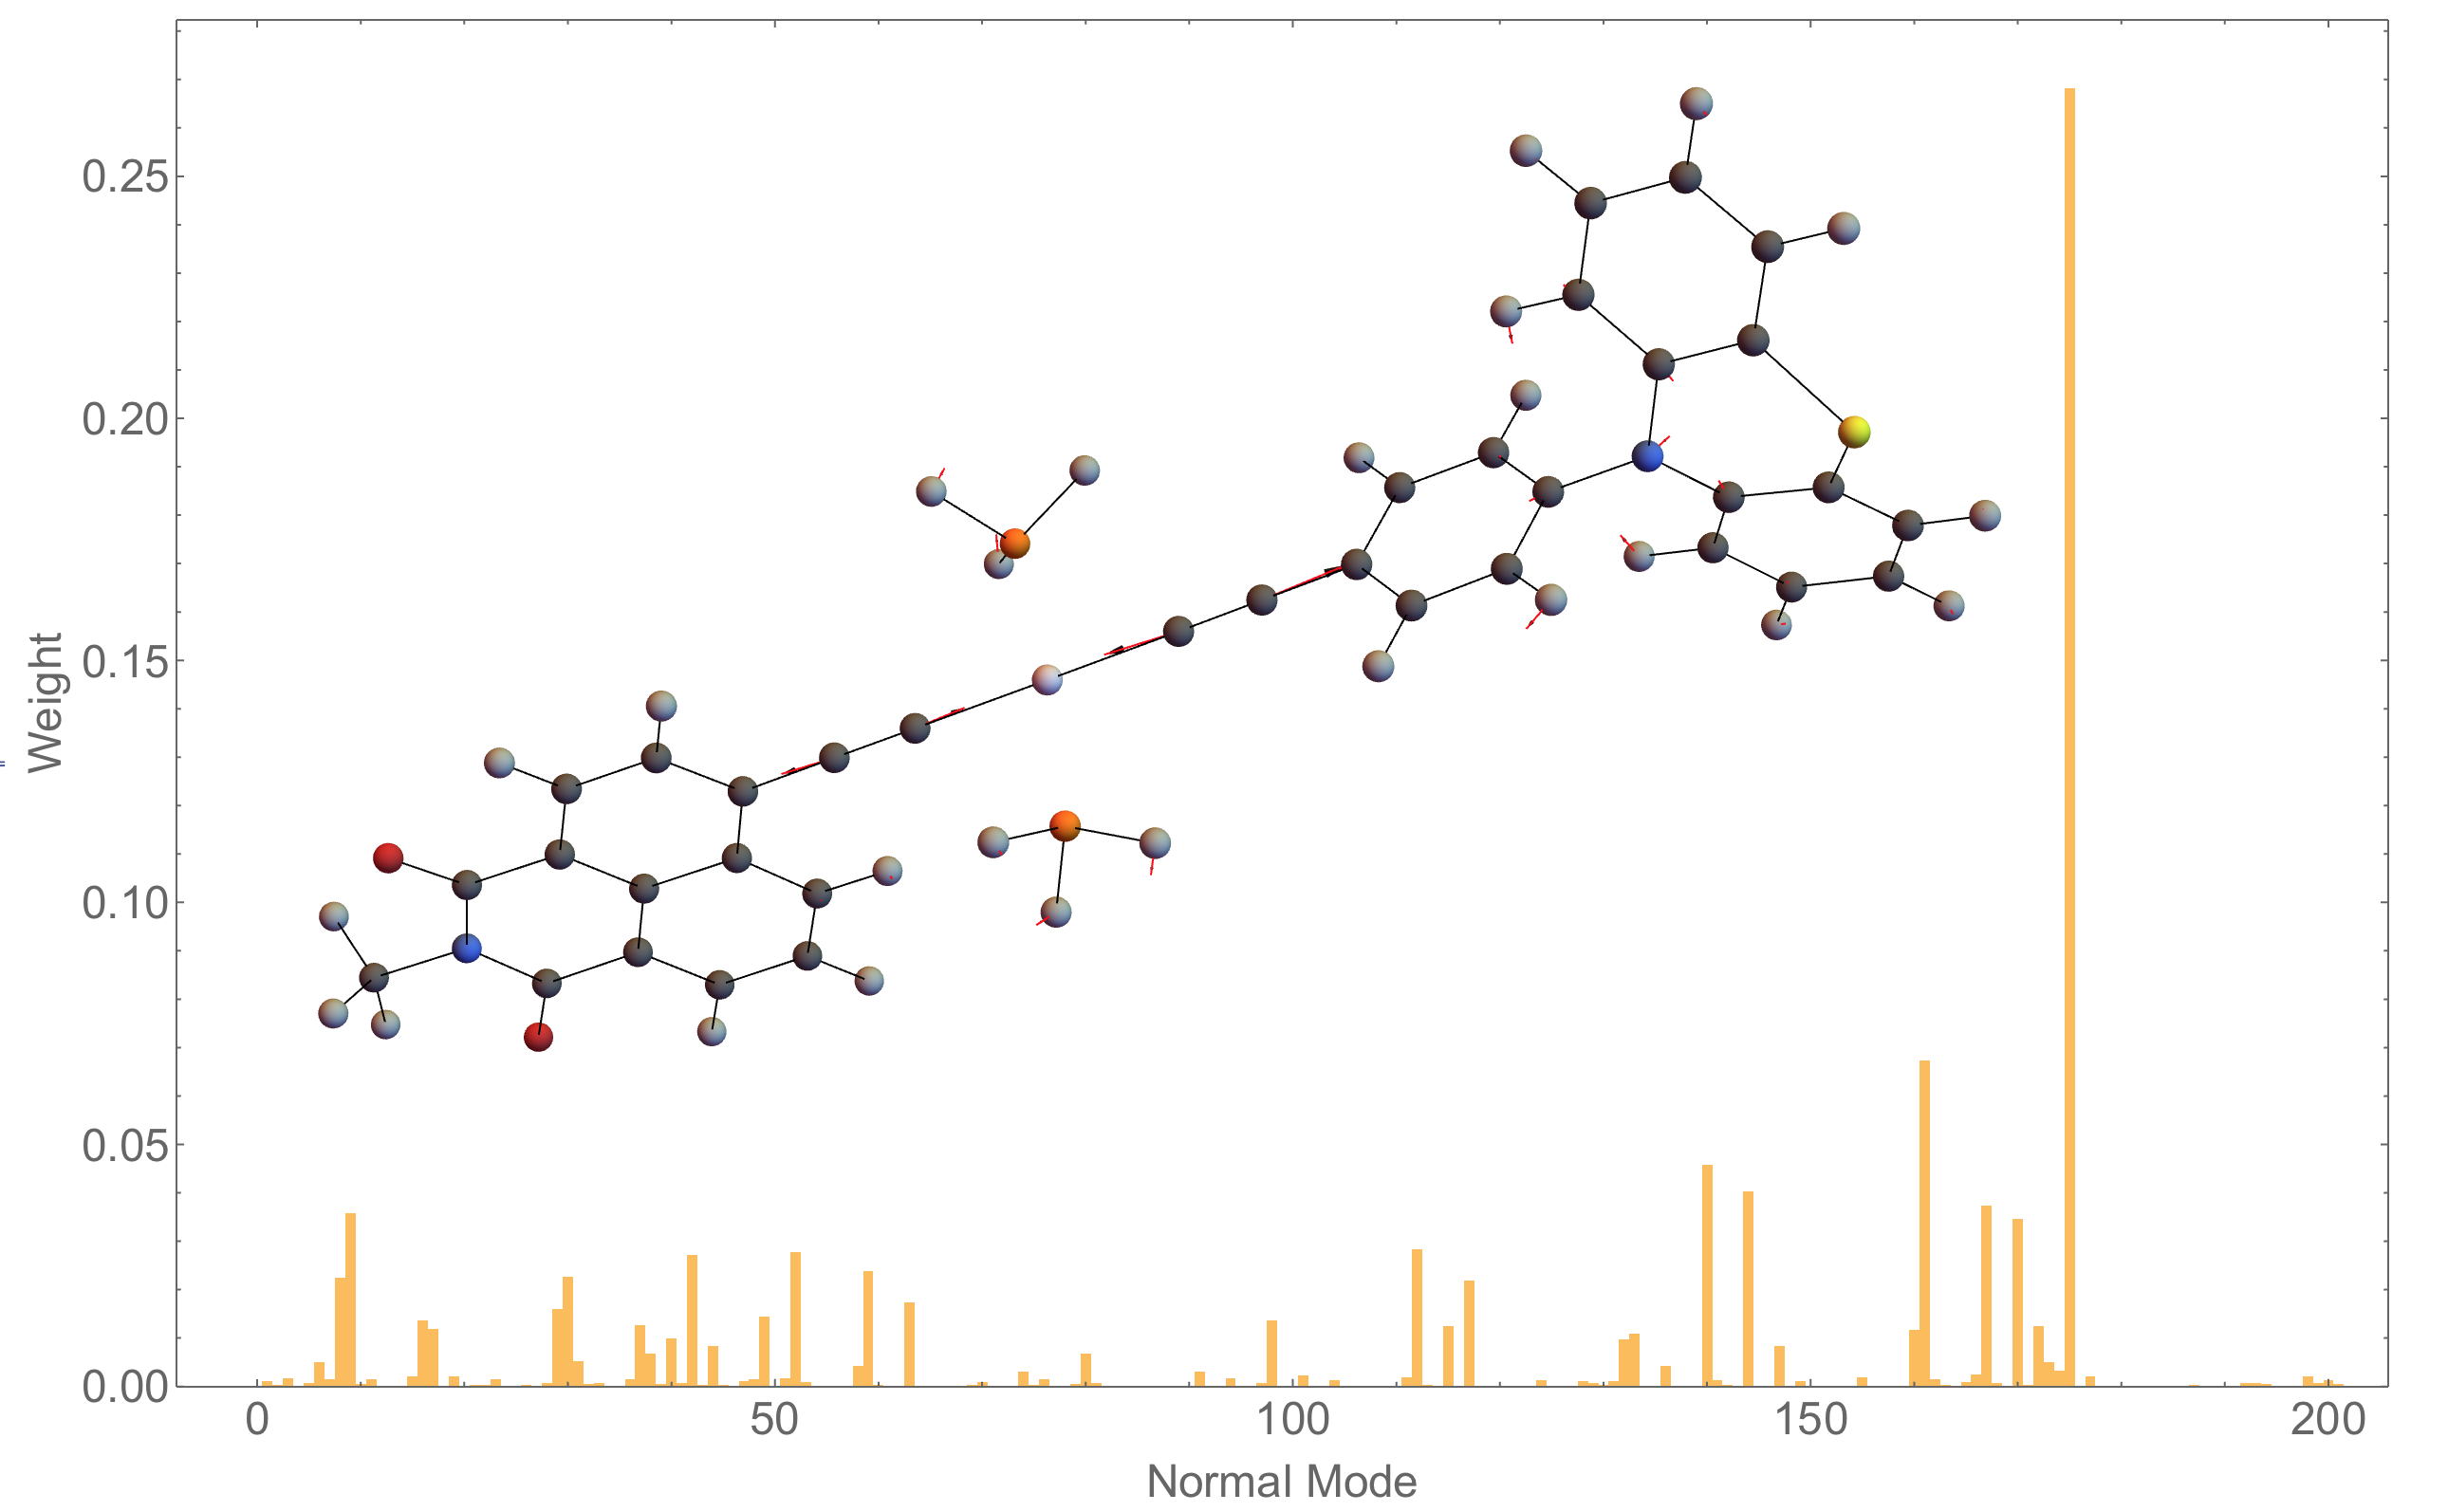
\includegraphics[width=0.88\columnwidth]{Chapters/chap4/Images/plmT32.png}}
\caption{
Projection of primary mode of (a) CSS $\rightarrow$ \textsuperscript{3}NAP, (b) CT $\rightarrow$ \textsuperscript{3}NAP calculated at \textsuperscript{3}NAP geometry onto the normal modes of \textsuperscript{3}NAP. Embedded molecule shows the atomic displacement vectors of primary mode. If we focus on the C$\equiv$C bonds, PLMs are like
PTZ-Ph-C$\equiv$C-Pt-C$\protect\overset{\longleftrightarrow}{\equiv}$C-NAP
in (a) and
PTZ-Ph-$\protect\overset{\longleftarrow}{C}\equiv\protect\overset{\longrightarrow}{C}$-Pt-$\protect\overset{\longrightarrow}{C}\equiv\protect\overset{\longleftarrow}{C}$-NAP
in (b).}\label{projT1}
\end{figure}

\begin{figure}[]
% \subfloat[]{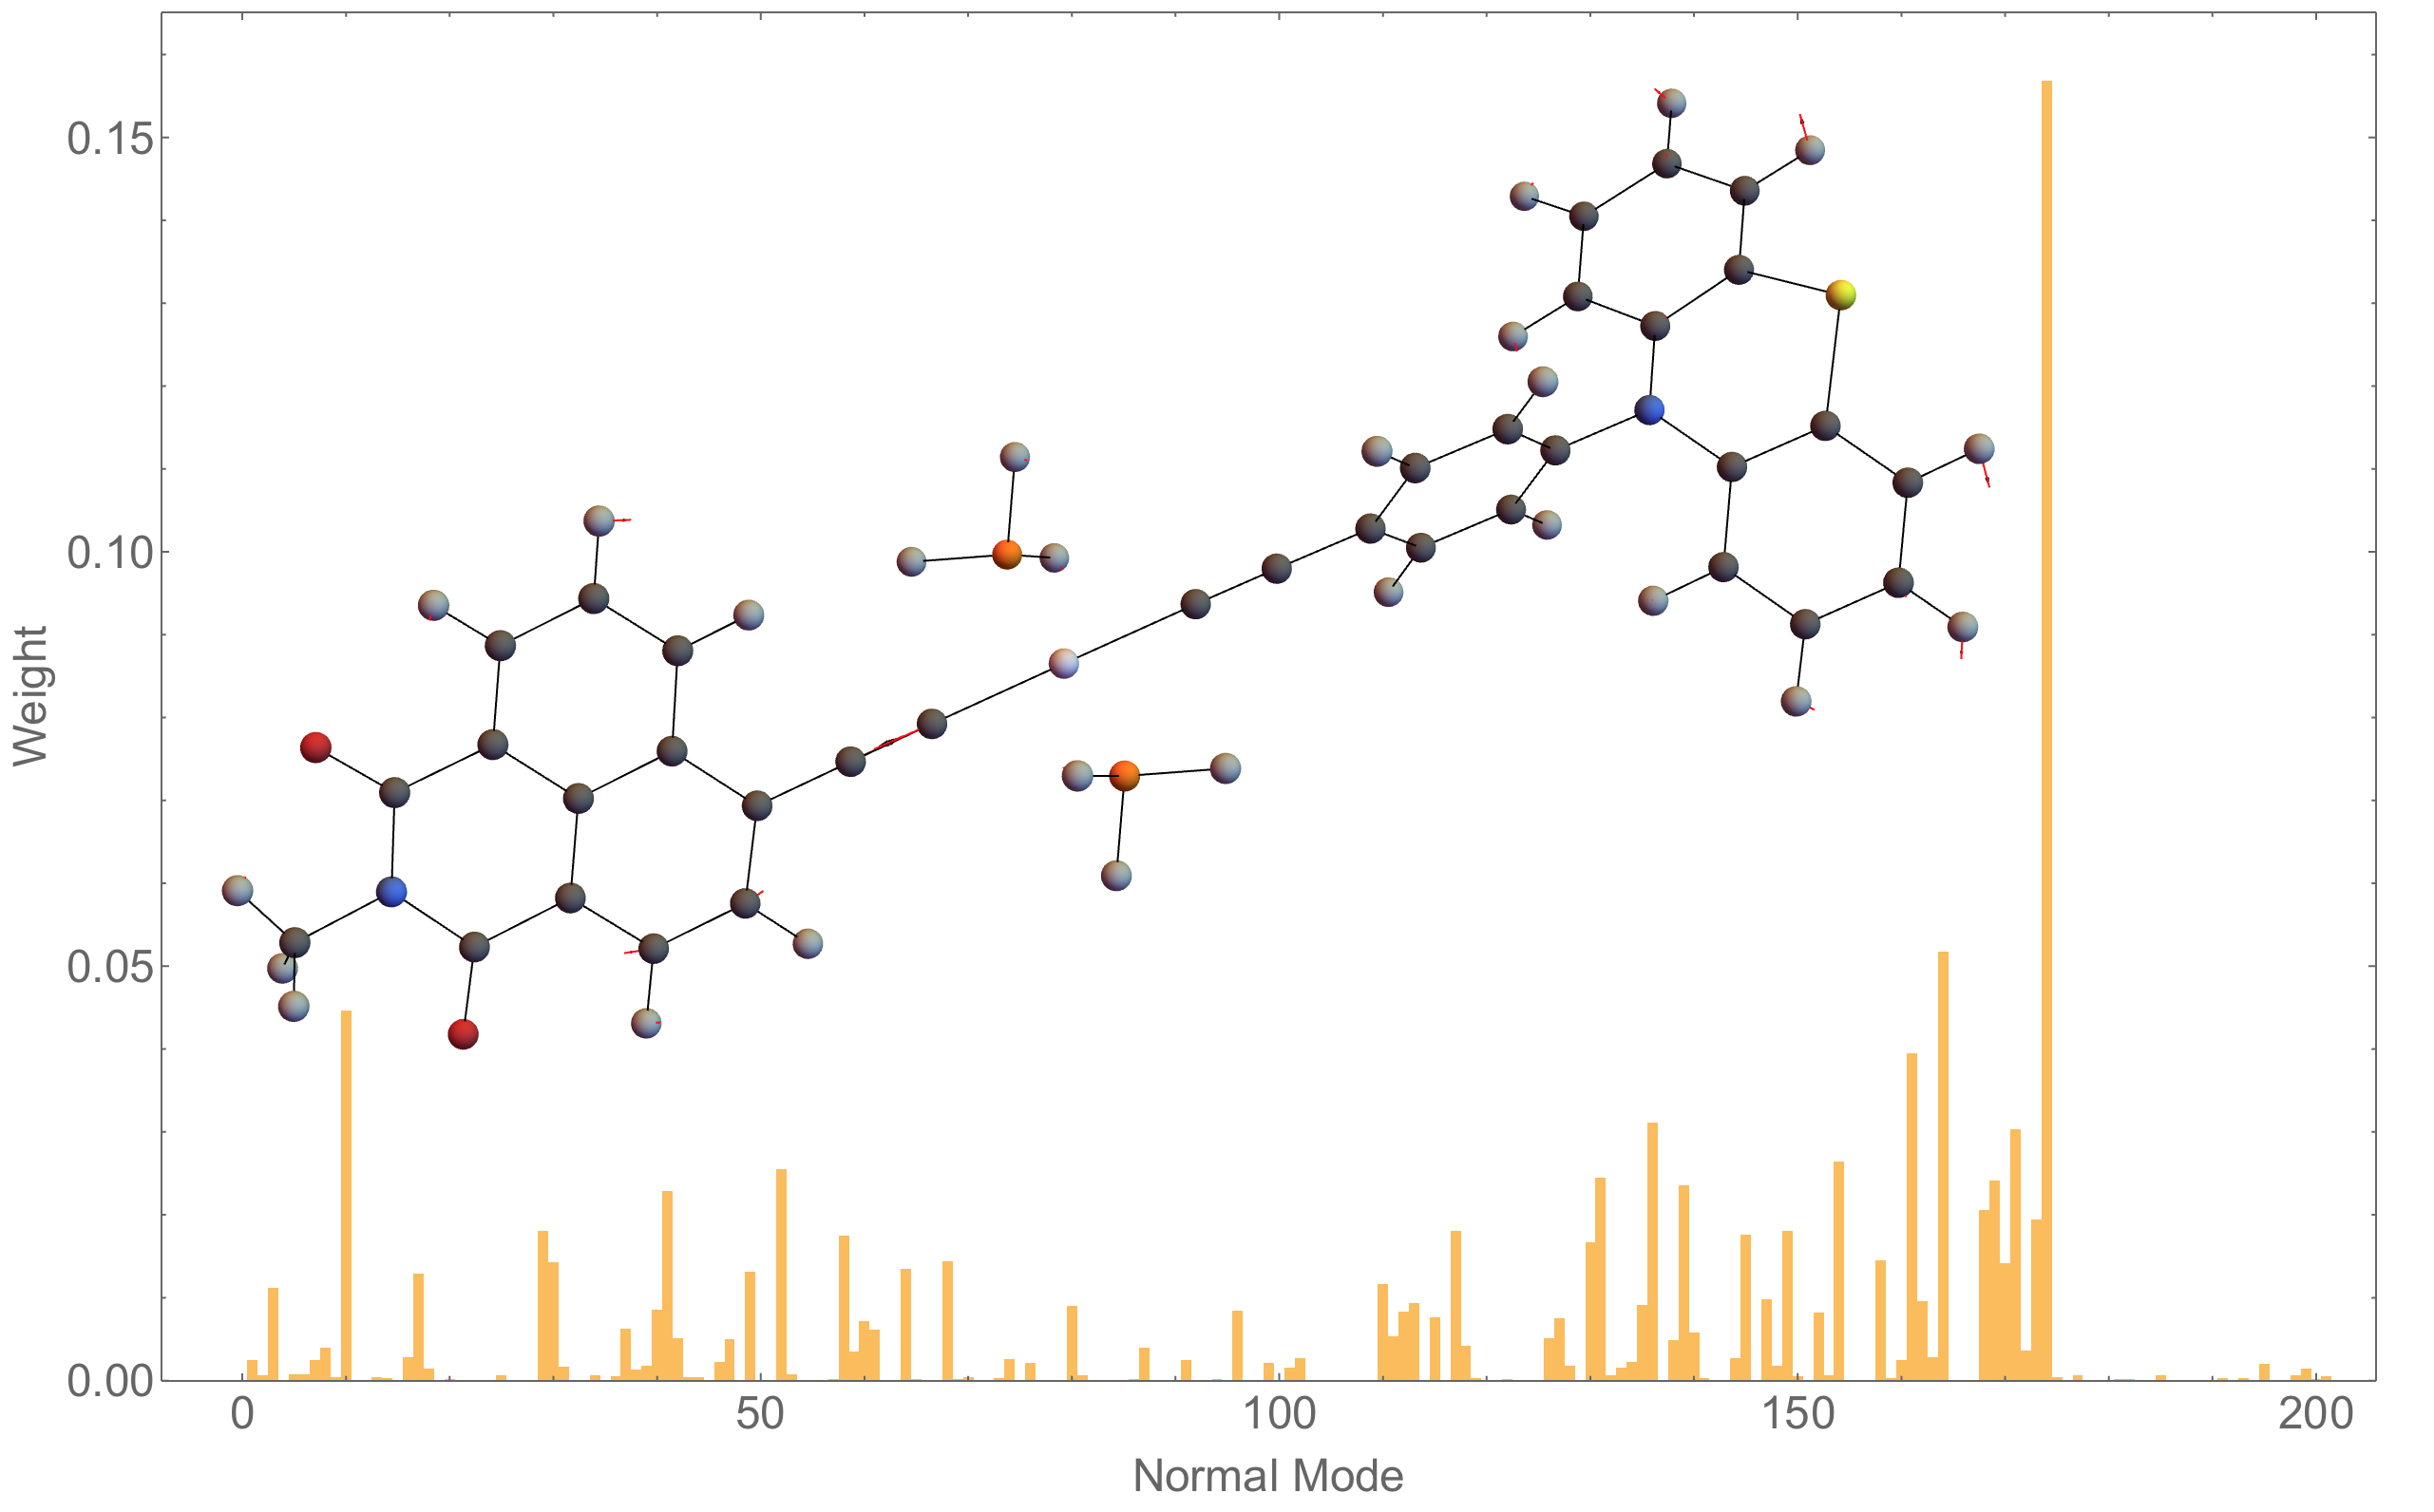
\includegraphics[width=0.89\columnwidth]{Chapters/chap4/Images/plmT12.png}}\\
% \subfloat[]{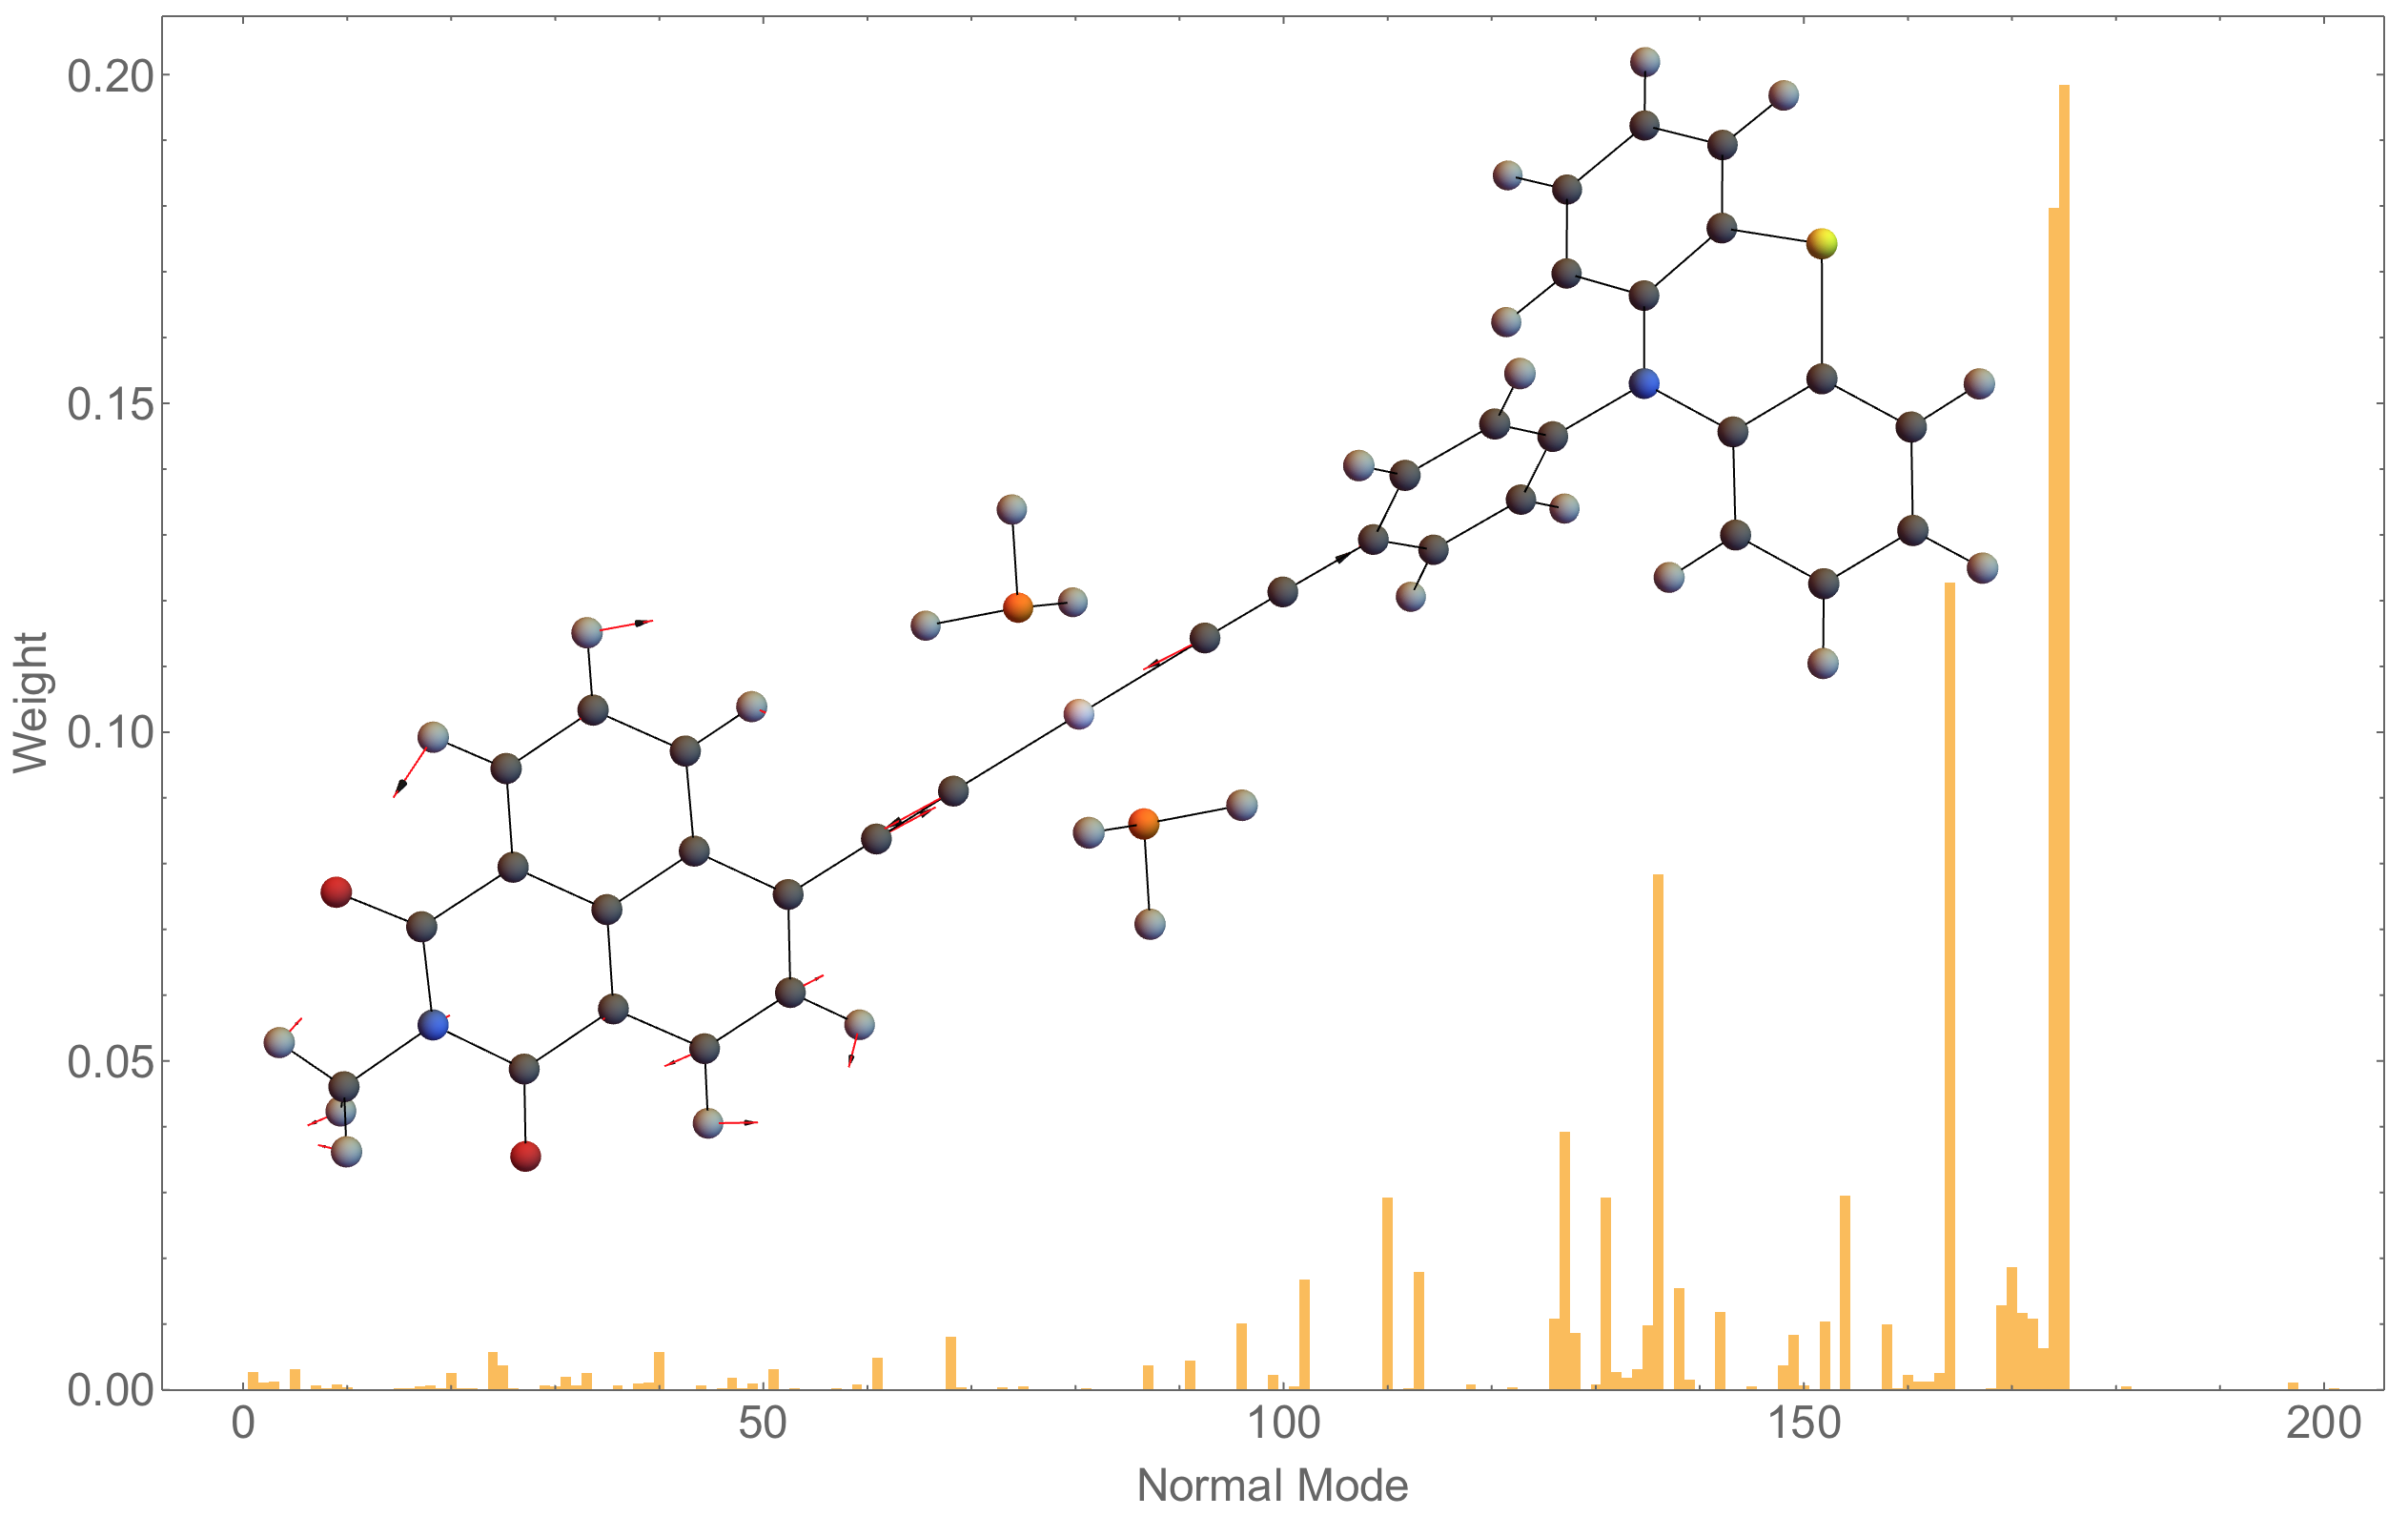
\includegraphics[width=0.89\columnwidth]{Chapters/chap4/Images/plmT13.png}}
\subfloat[]{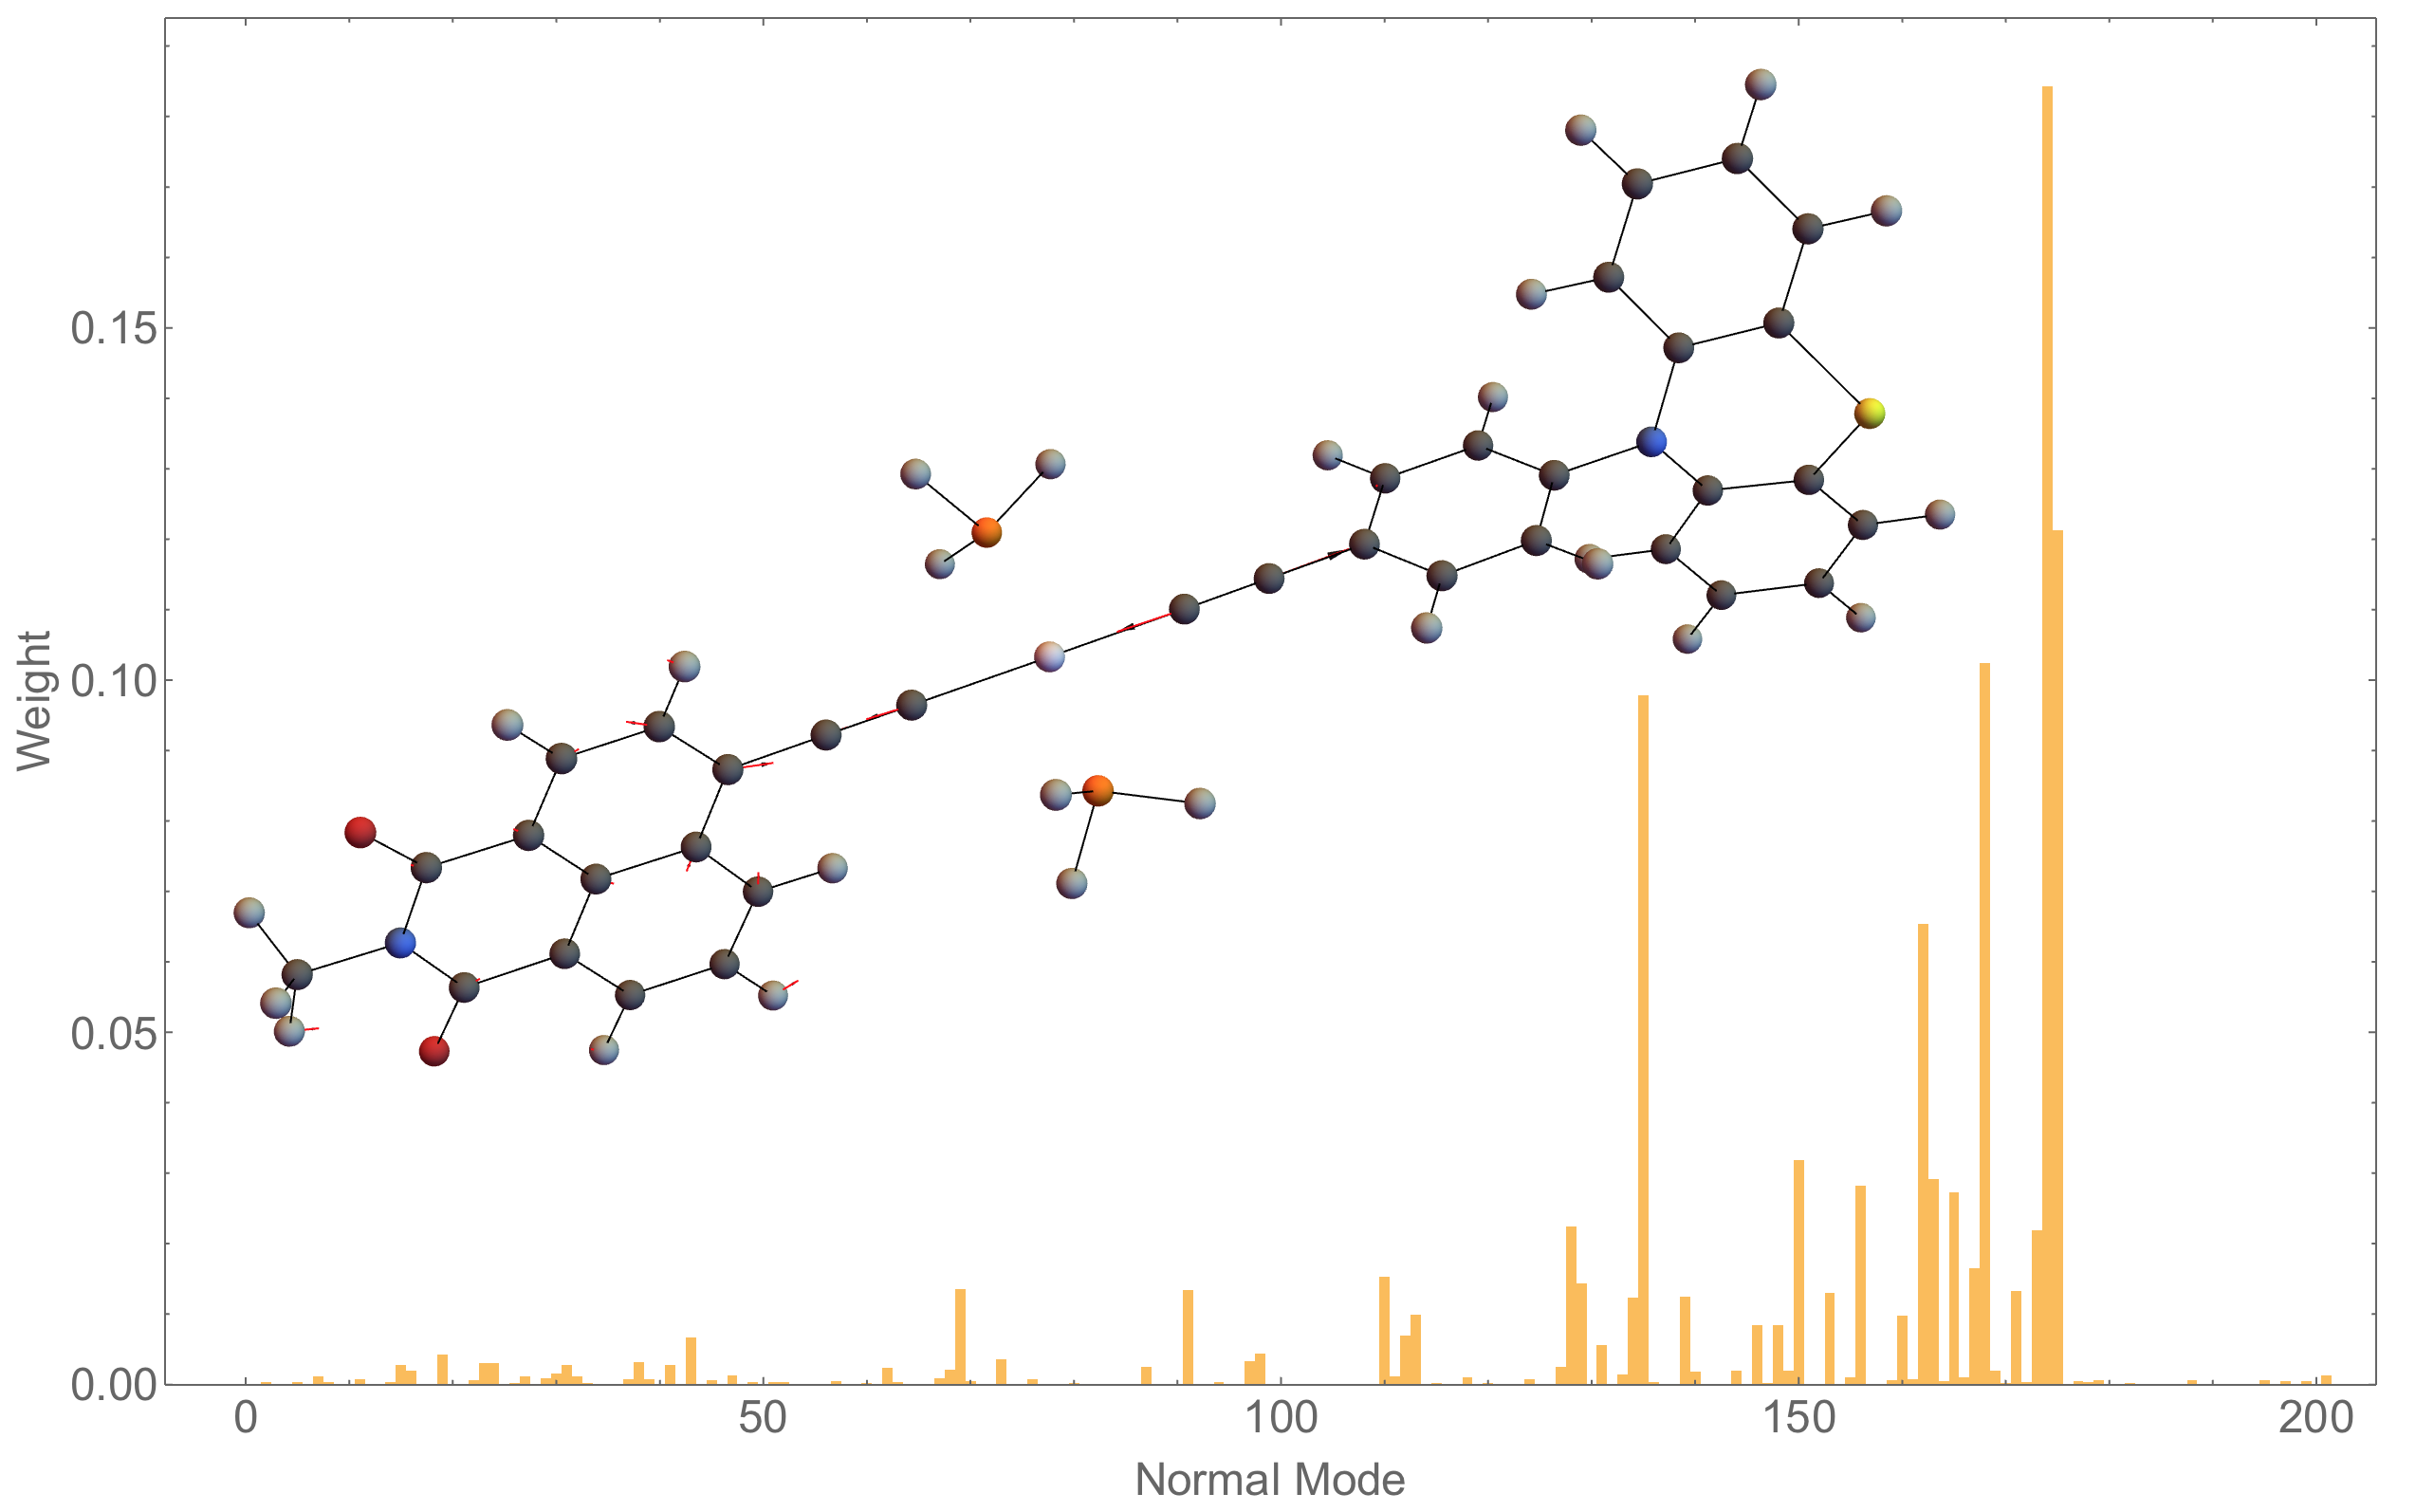
\includegraphics[width=0.85\columnwidth]{Chapters/chap4/Images/plmT31.png}}\\
\subfloat[]{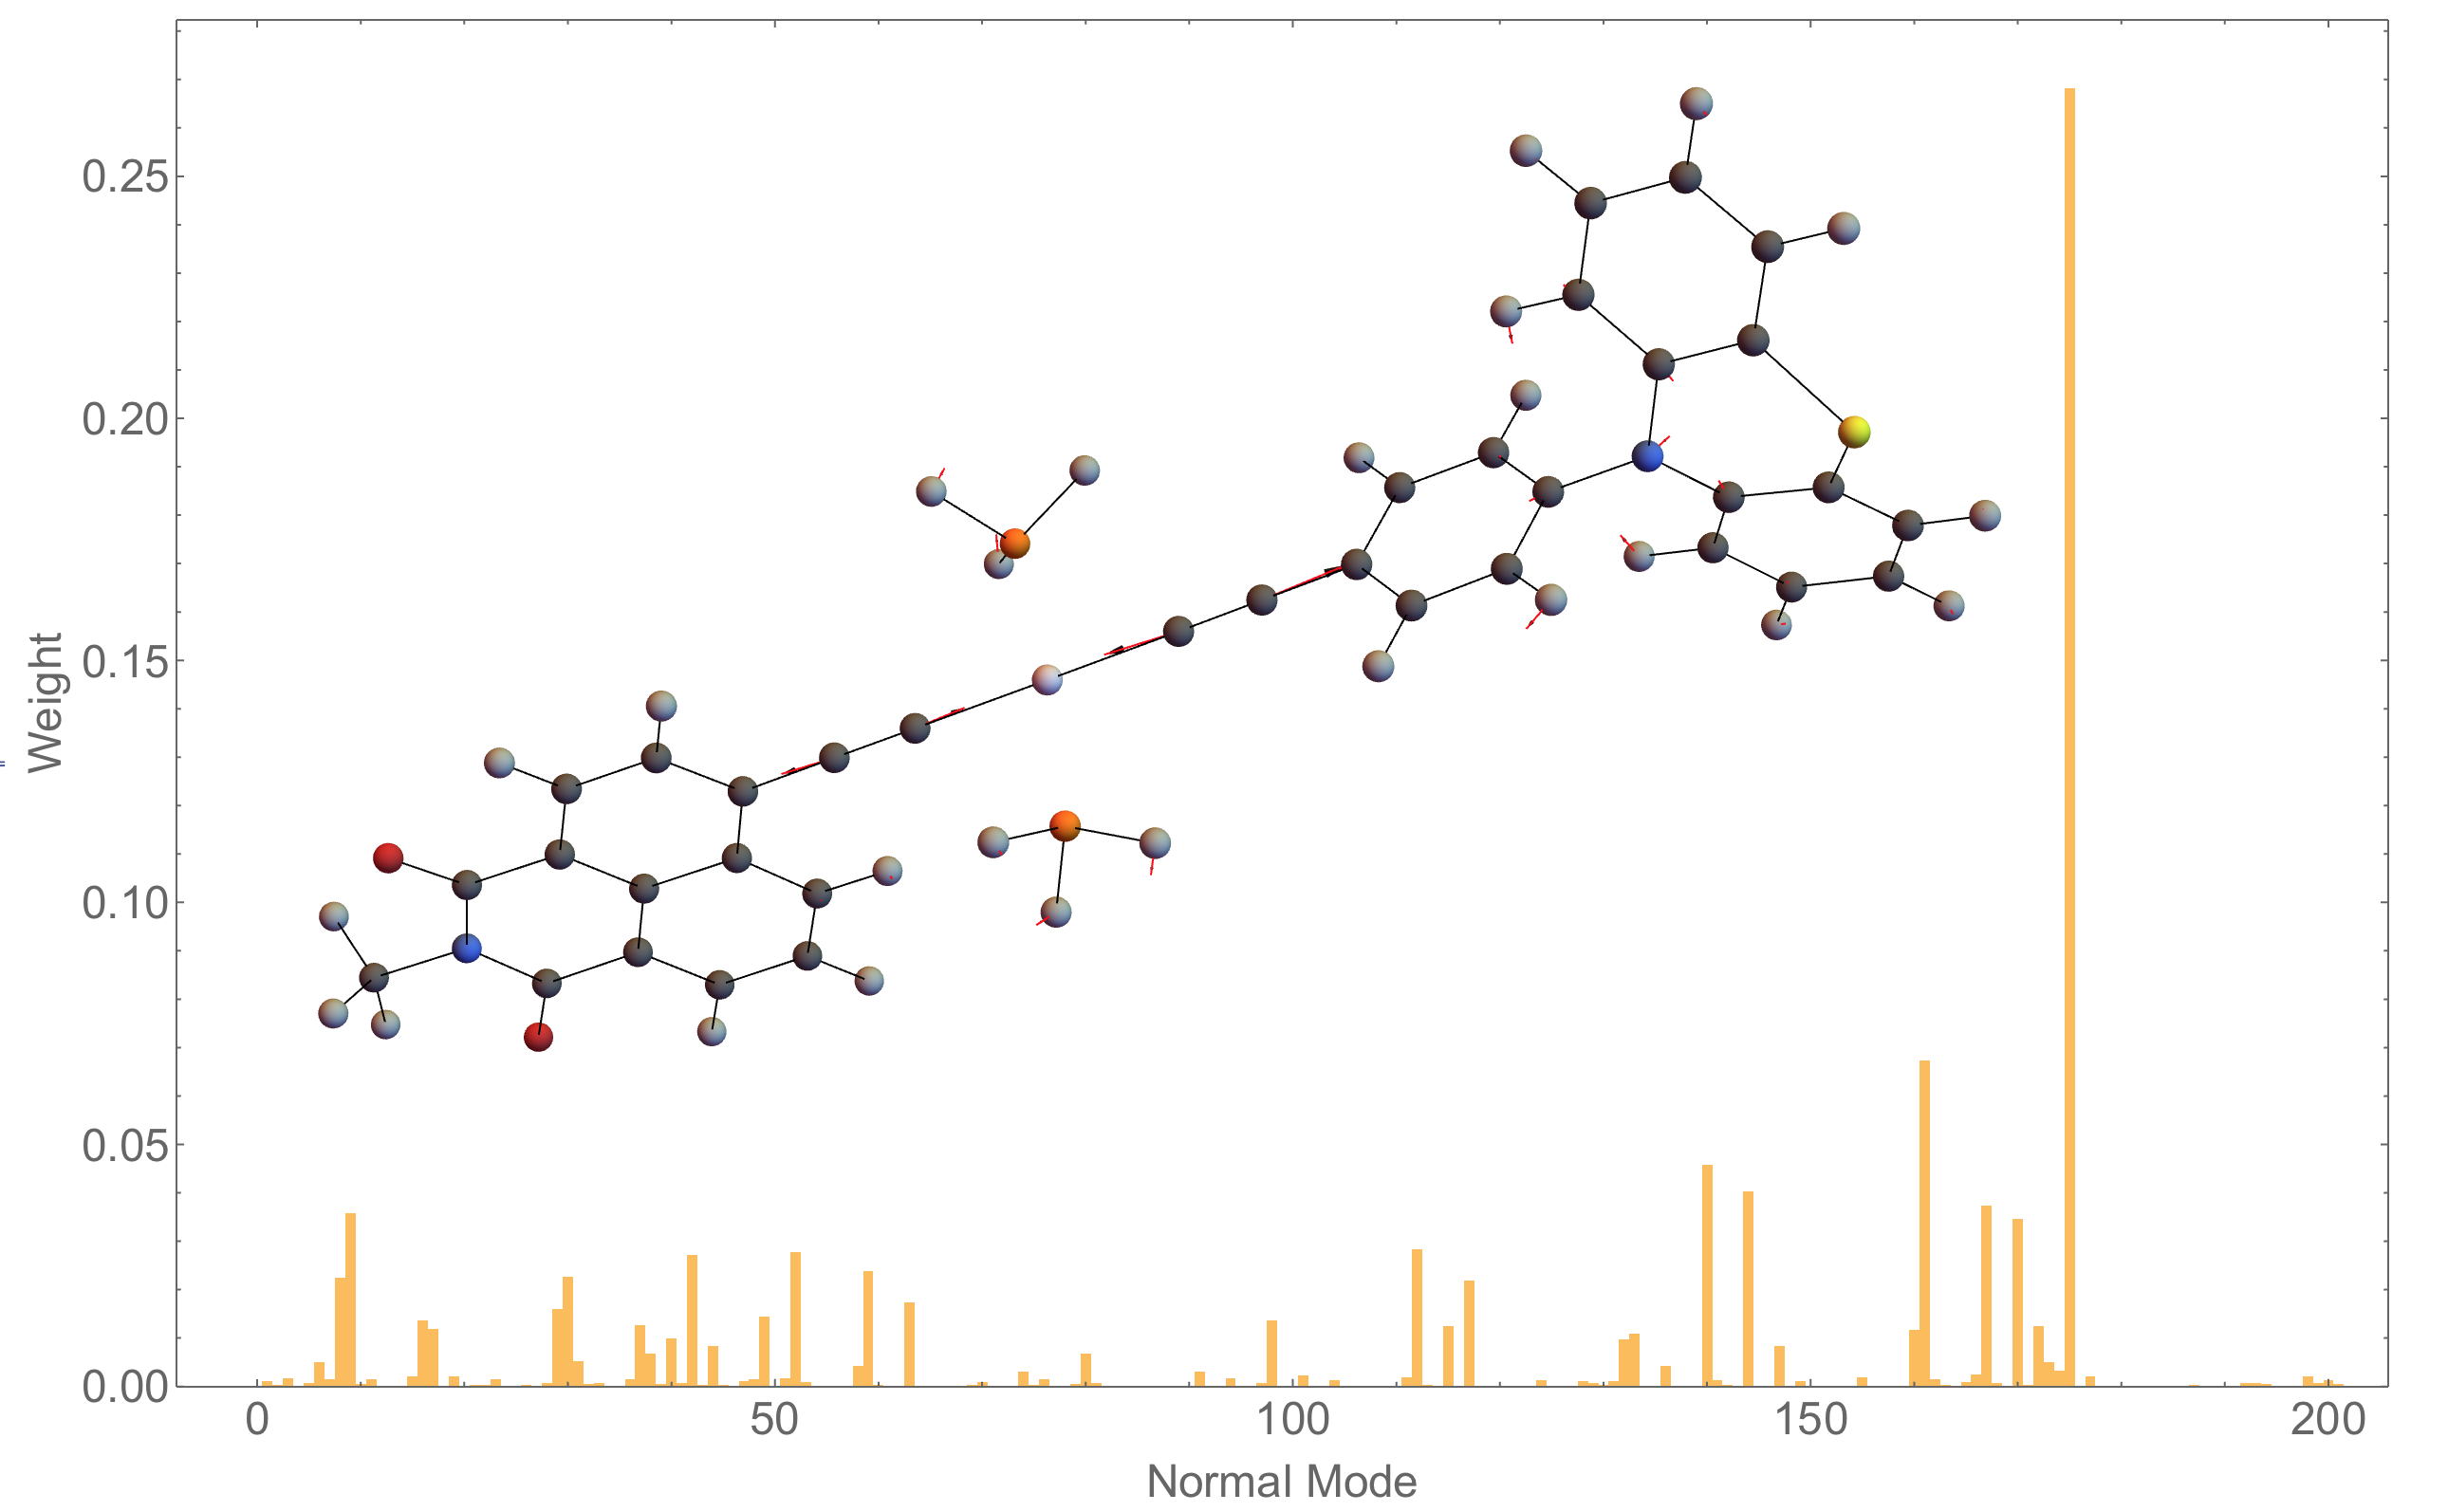
\includegraphics[width=0.85\columnwidth]{Chapters/chap4/Images/plmT32.png}}
\caption{
Projection of primary mode of (a) CT $\rightarrow$ \textsuperscript{3}NAP, and (b) CT $\rightarrow$ CSS calculated at CT geometry onto the normal modes of CT. Embedded molecule shows the atomic displacement vectors of primary mode. If we focus on the C$\equiv$C bonds, PLMs are like
PTZ-Ph-$\protect\overset{\longleftarrow}{C}\equiv\protect\overset{\longrightarrow}{C}$-Pt-$\protect\overset{\rightarrow}{C}\equiv\protect\overset{\leftarrow}{C}$-NAP
in (a) and
PTZ-Ph-$\protect\overset{\longleftarrow}{C}\equiv\protect\overset{\longrightarrow}{C}$-Pt-$\protect\overset{\leftarrow}{C}\equiv\protect\overset{\rightarrow}{C}$-NAP
in (b).
}\label{projT3}
\end{figure}


\begin{figure}[]
\subfloat{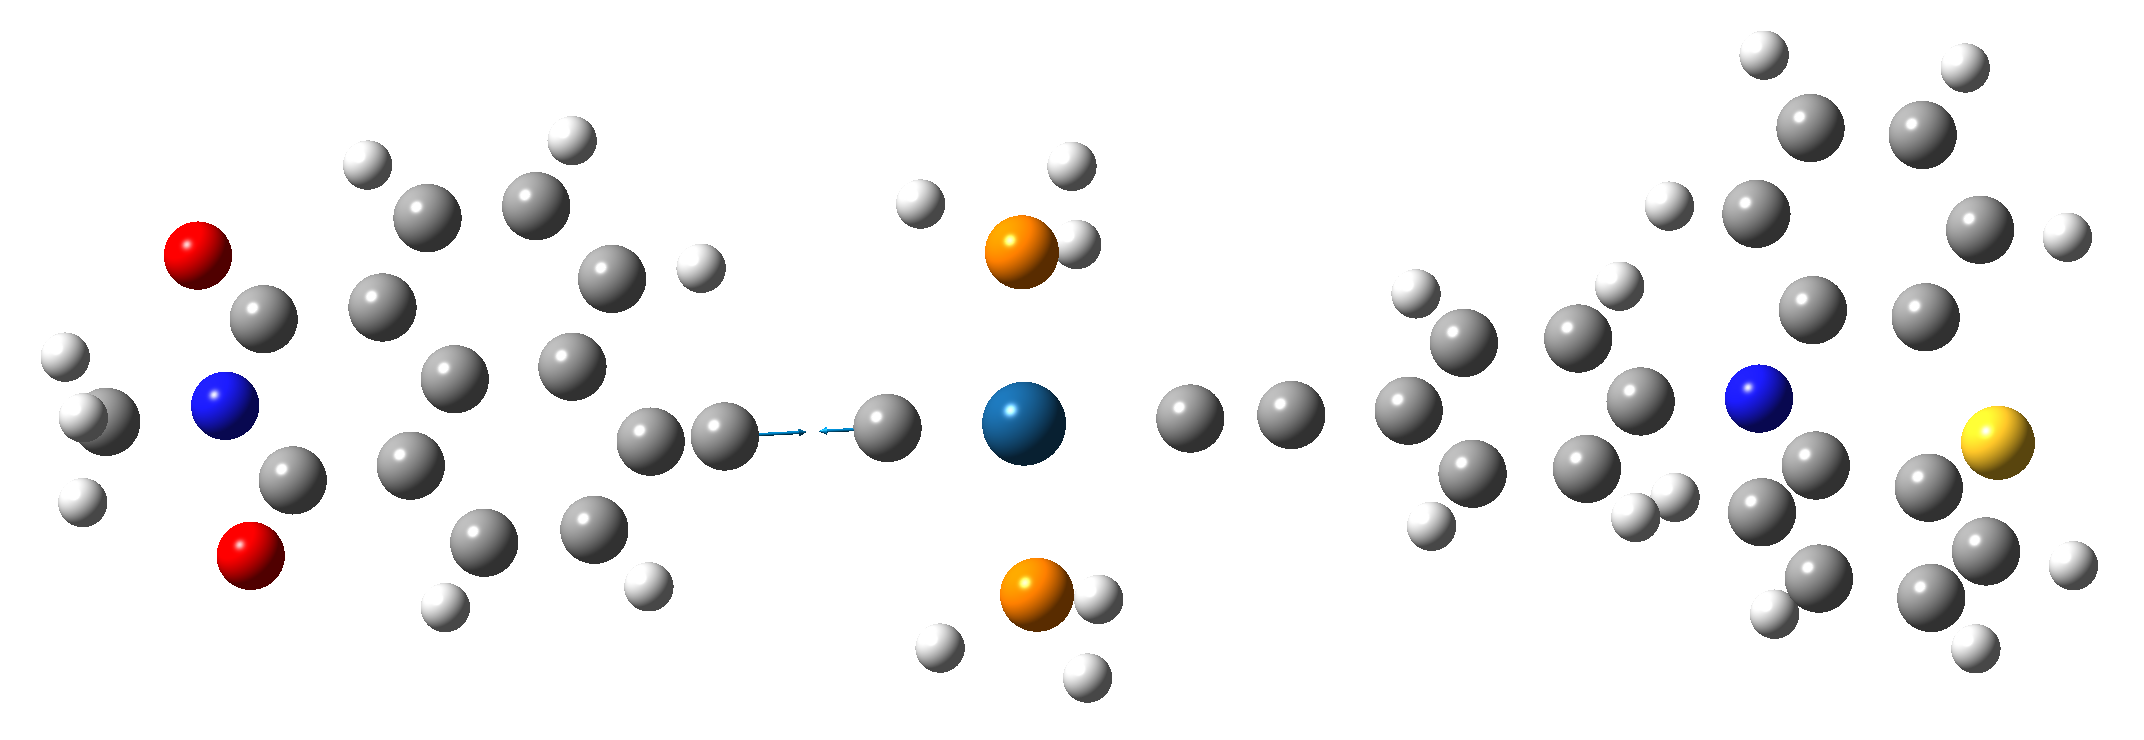
\includegraphics[width=0.85\columnwidth]{Chapters/chap4/Images/t1_174.png}}\\
\subfloat{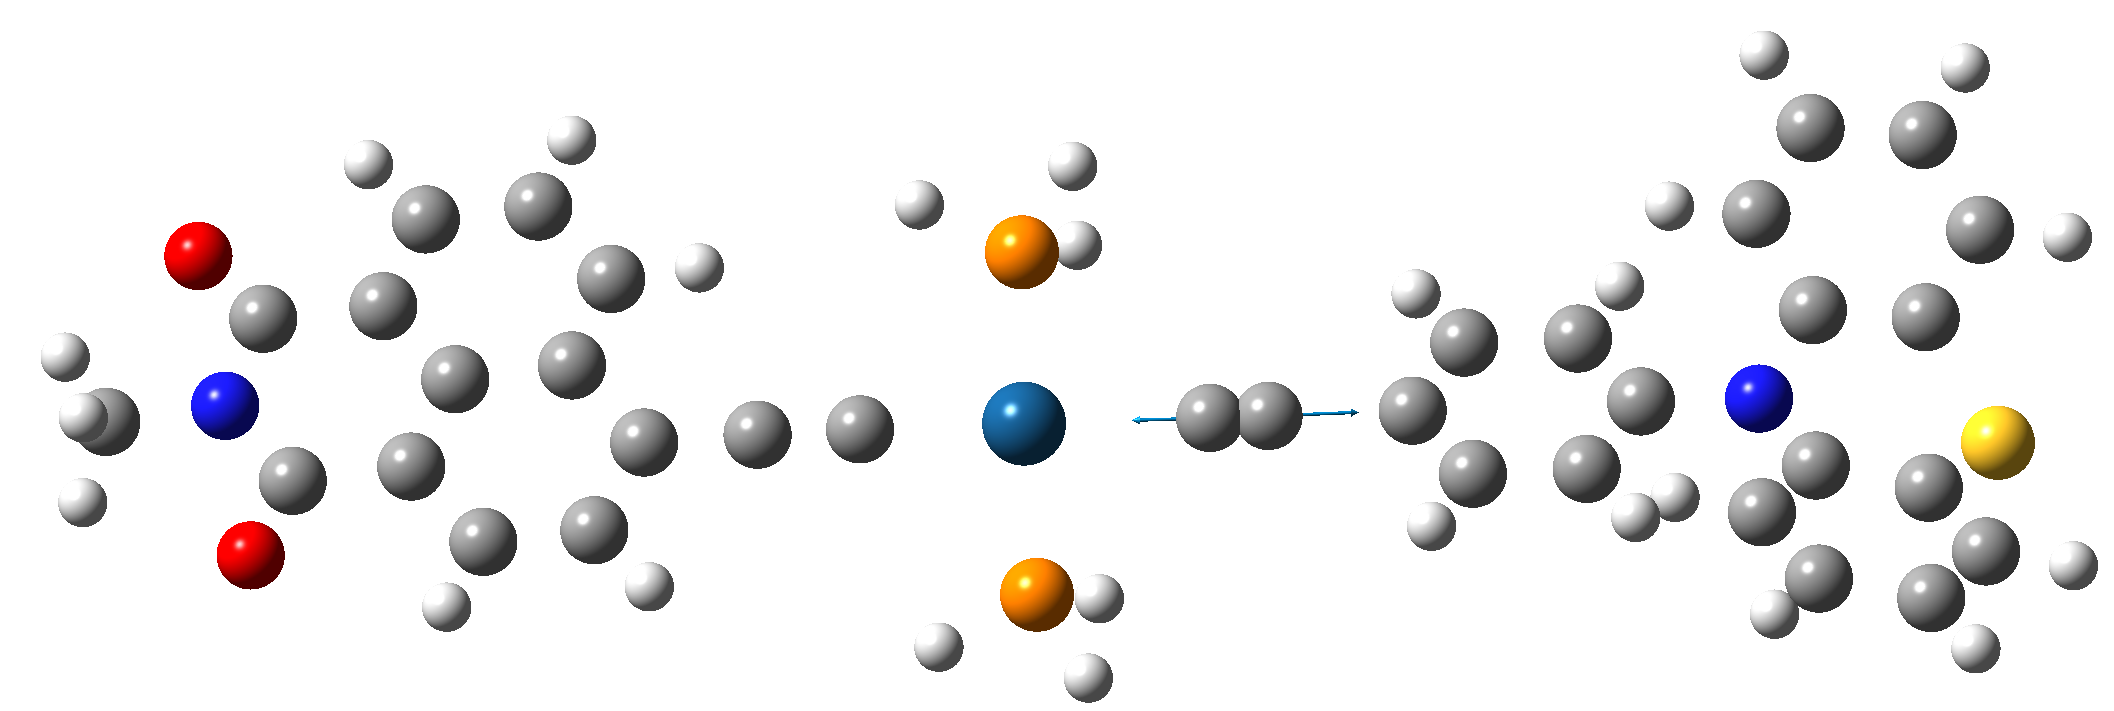
\includegraphics[width=0.85\columnwidth]{Chapters/chap4/Images/t1_175.png}}\\
\subfloat{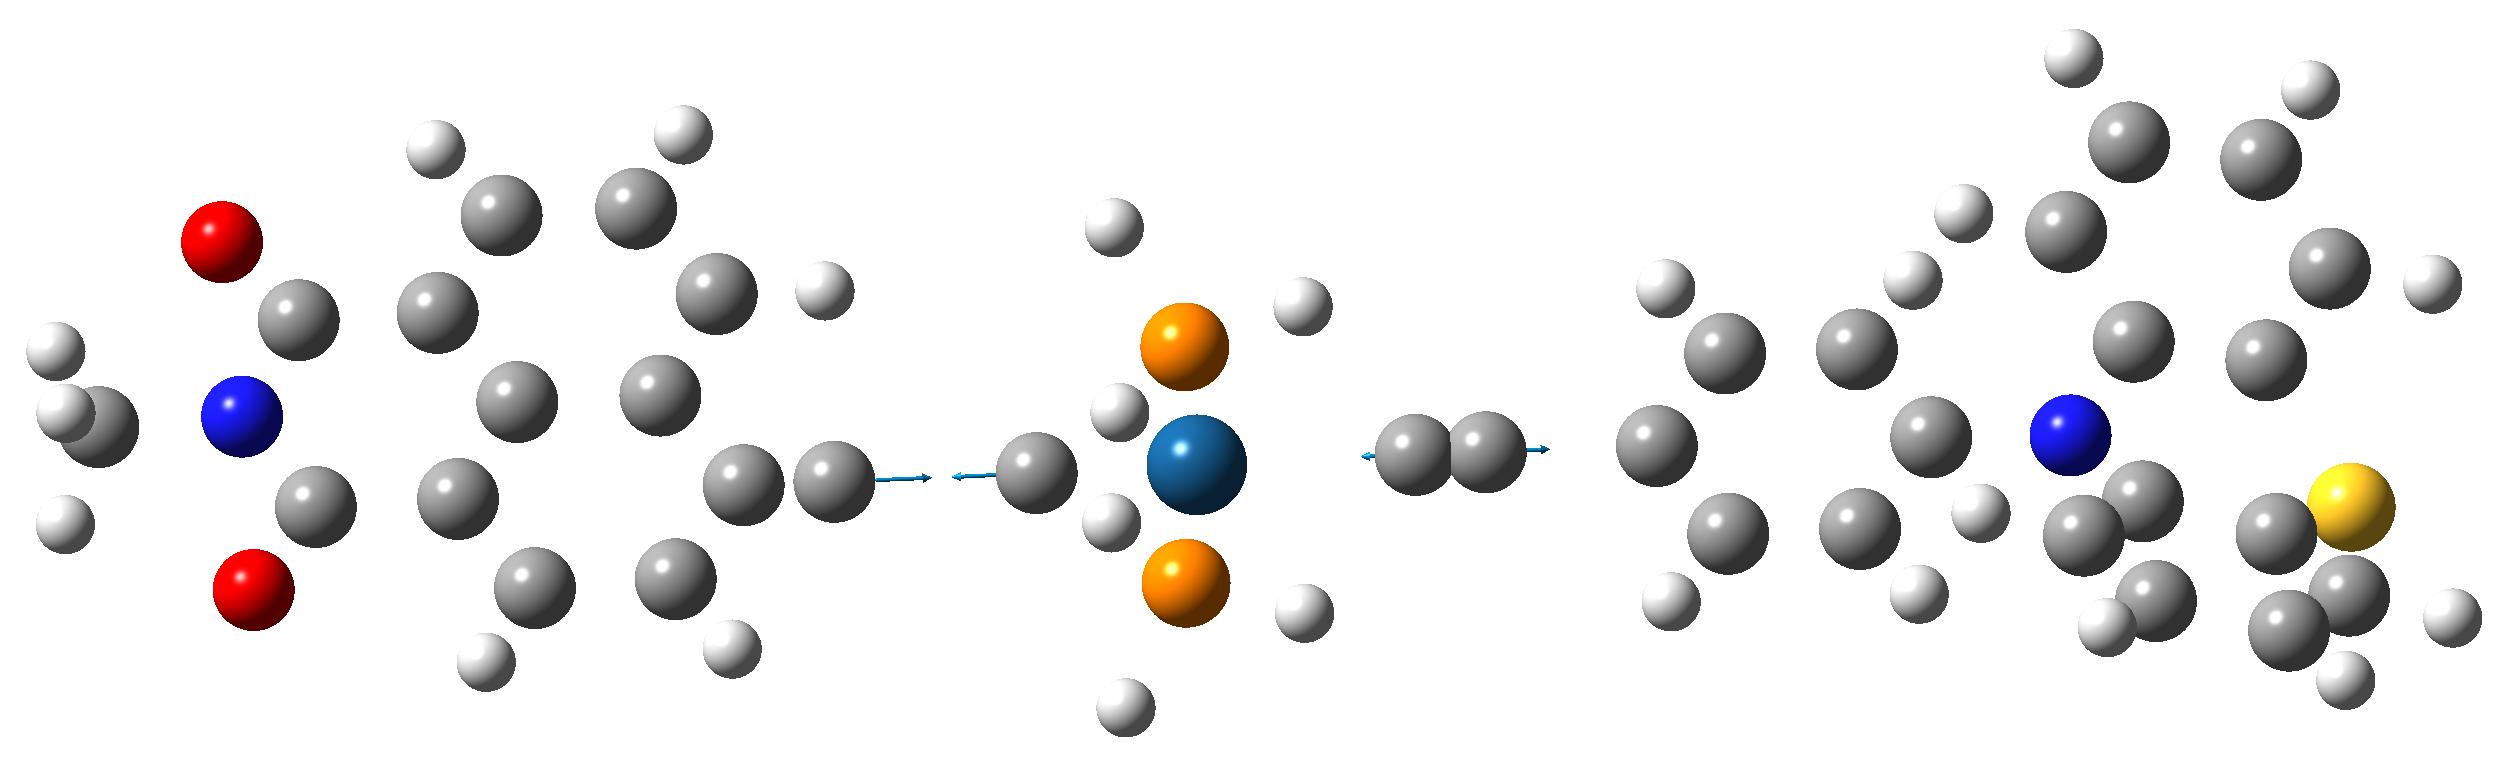
\includegraphics[width=0.85\columnwidth]{Chapters/chap4/Images/t3_174.png}}\\
\subfloat{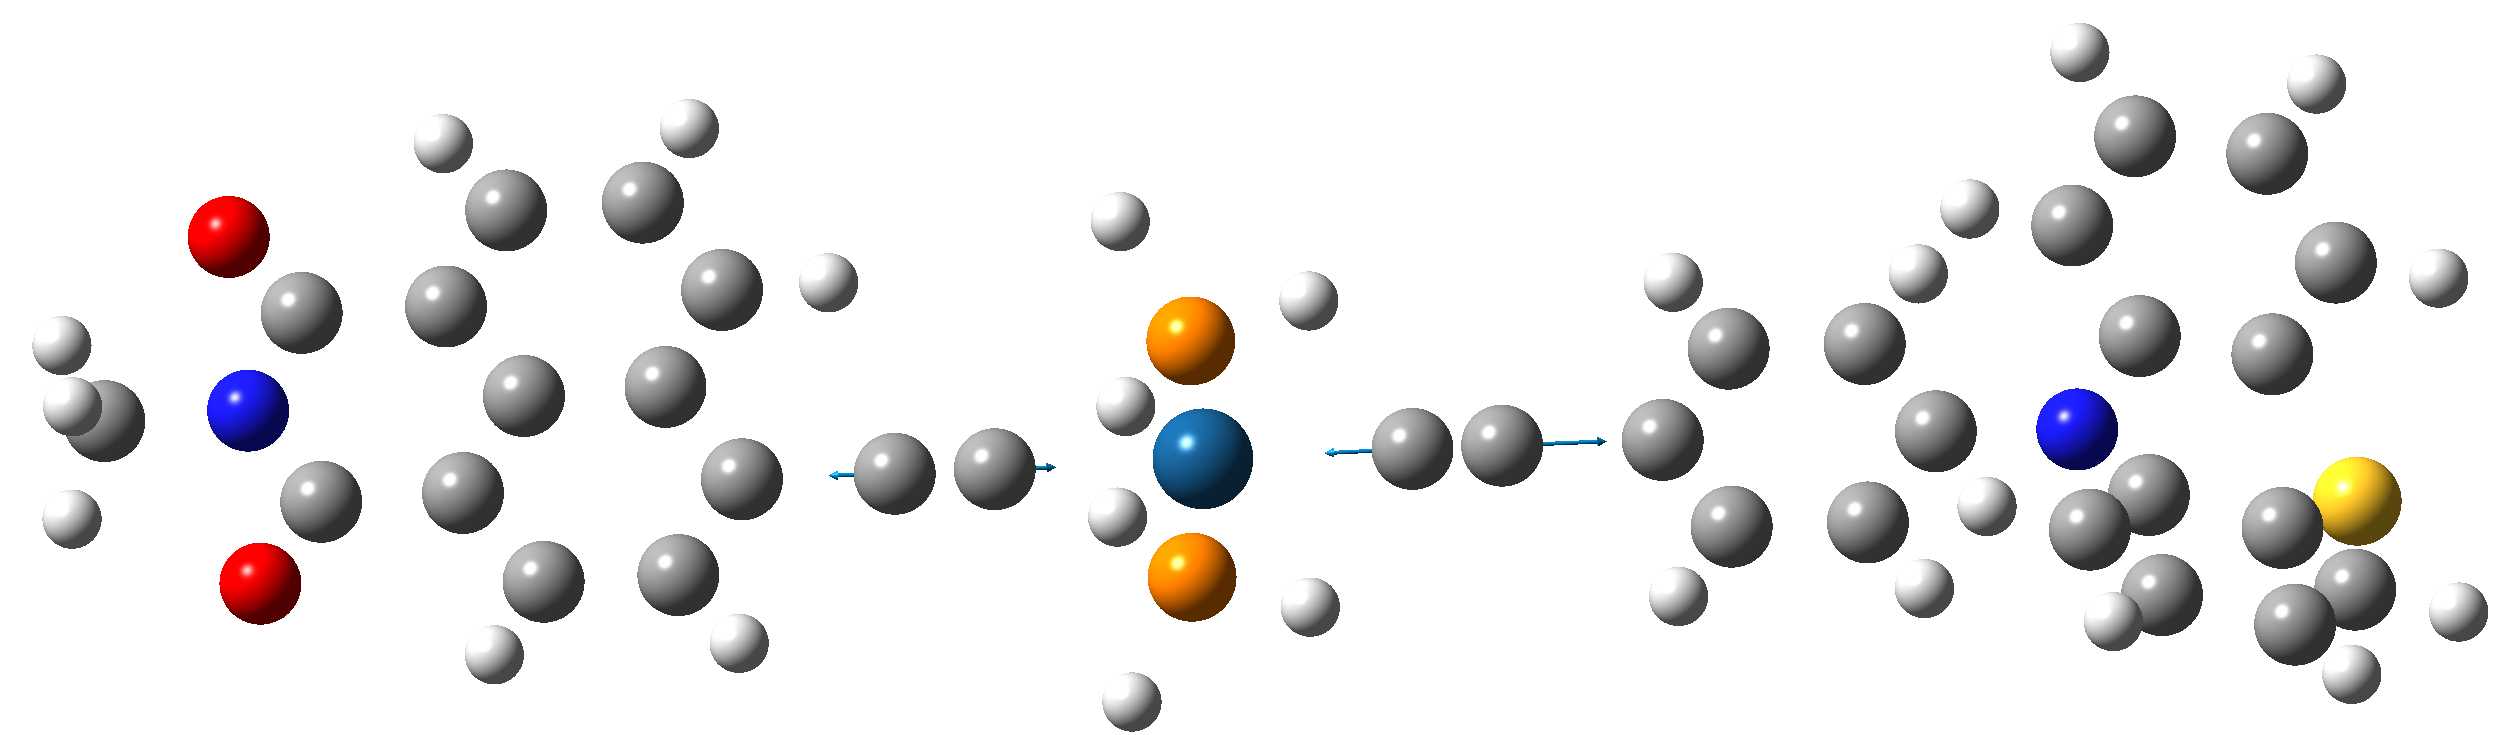
\includegraphics[width=0.85\columnwidth]{Chapters/chap4/Images/t3_175.png}}
\caption{From top to bottom: the displacement vectors of the 174th, 175th mode of \textsuperscript{3}NAP state, the 174th, 175th mode of CT state. For clarity, bonds are not shown. They are all the stretching modes of single C$\equiv$C bond, look like
PTZ-Ph-C$\equiv$C-Pt-C$\protect\overset{\longleftrightarrow}{\equiv}$C-NAP in (a),
PTZ-Ph-C$\protect\overset{\longleftrightarrow}{\equiv}$C-Pt-C$\equiv$C-NAP in (b),
PTZ-Ph-$\protect\overset{\leftarrow}{C}\equiv\protect\overset{\rightarrow}{C}$-Pt-$\protect\overset{\longrightarrow}{C}\equiv\protect\overset{\longleftarrow}{C}$-NAP
 in (c), and
PTZ-Ph-$\protect\overset{\longleftarrow}{C}\equiv\protect\overset{\longrightarrow}{C}$-Pt-$\protect\overset{\leftarrow}{C}\equiv\protect\overset{\rightarrow}{C}$-NAP
 in (d).
}\label{NMT1T3}
\end{figure}



As experiments show that the excitation of C$\equiv$C bond radically affected the ET process, we expect the triple bond vibration to dominate the primary modes, at least for the CT state based calculations, since they achieve good agreement. Fig. \ref{projT1} and \ref{projT3} show the projection of primary modes onto the normal modes of corresponding state, {\em i.~e.}, the primary modes calculated at CT geometry are projected onto the normal modes of the CT state, and those at \textsuperscript{3}NAP are projected onto \textsuperscript{3}NAP's normal modes. It turns out that all four primary modes involve obvious C$\equiv$C displacement, and it is verified by the projections. The projections of primary modes are dominated by 1 or 2 normal modes. In Fig. \ref{projT1}(a), it is the 174th normal mode (ordered by increasing frequency) that dominates; in Fig. \ref{projT1}(b), the 174th and 175th modes dominate. Similarly, 174th and 175th modes dominate in Fig. \ref{projT3}(a) and  175th mode in Fig. \ref{projT3}(b).

All these normal modes are C$\equiv$C stretching modes, as shown in Fig. \ref{NMT1T3}. We suggest that the primary mode of  CT $\rightarrow$ CSS transition (Fig. \ref{projT3}(b)) is the one involves C$\equiv$C vibration most. It has a component which has the largest weight, > 0.25, in all four primary modes. And that component clearly dominates other normal modes. Experimentally, after the IR pump is applied, the CT $\rightarrow$  \textsuperscript{3}NAP transition is relatively accelerated compared to the CT $\rightarrow$ CSS transition. By comparing the primary modes of the two transitions at CT geometry, we see that the primary mode of CT $\rightarrow$  \textsuperscript{3}NAP transition  is mainly antisymmetric stretching of two C$\equiv$C bonds, while that of CT $\rightarrow$ CSS transition is symmetric. As a result, the primary mode of CT $\rightarrow$  \textsuperscript{3}NAP is more IR active than that of CT $\rightarrow$ CSS transition. It may explain why CT $\rightarrow$  \textsuperscript{3}NAP  transition is relatively accelerated with IR pump.
% As for PTZ-CH\textsubscript{2}-Pt-NAP, the CT $\rightarrow$ CSS step can be fully switched off by vibronic excitation, the step is supposed to be the one influenced by C$\equiv$C stretching most. Although PTZ-Pt-NAP does not show such radical change, we expect the the CT $\rightarrow$ CSS to be the most C$\equiv$C involved, as two molecules only differ by a -CH\textsubscript{2}-

% section results (end)





\subsection{Condon Approximation}\label{sec:condon}

As mentioned above, the results at the CT state, including rate constant and projected modes, are satisfactory, while those at the \textsuperscript{3}NAP state are poor. The reason is complex. Here we illustrate that the break down of Condon approximation may be one of the causes.


Our model explicitly relies on two assumptions, parabolic assumption and Condon approximation. Parabolic assumption assumes potential energy surface (PES) is parabolic. For this molecule, parabolic assumption is probably true, as the PES has been shown to be parabolic along C$\equiv$C bond in Fig. \ref{PTZparabolas}. Condon approximation states that diabatic coupling is independent of nuclear coordinates, i.e., does not change when geometry changes. In Fig. \ref{interCondon} we show the change of diabatic coupling from the \textsuperscript{3}NAP state to the CT state. It is clear that diabatic couplings do undergo significant changes (note the y axis is logarithmic), especially in the CSS $\rightarrow$ \textsuperscript{3}NAP step, where the coupling can differ by two orders of magnitudes. General speaking, Condon approximation fails more near the \textsuperscript{3}NAP than near the CT state. It may explain why CT geometry gives better results.

To explore the effect of the change of diabatic coupling, we replace the original coupling with the average coupling along interpolation and redo the calculations. The new rate constants are illustrated in Fig. \ref{rateComp}, as ``with mean V''. The correction brings significant improvements, to both the Marcus and TCLME approaches, at the \textsuperscript{3}NAP geometry, especially for the most poorly computed  CSS $\rightarrow$ \textsuperscript{3}NAP transfer.

\begin{figure*}[t]
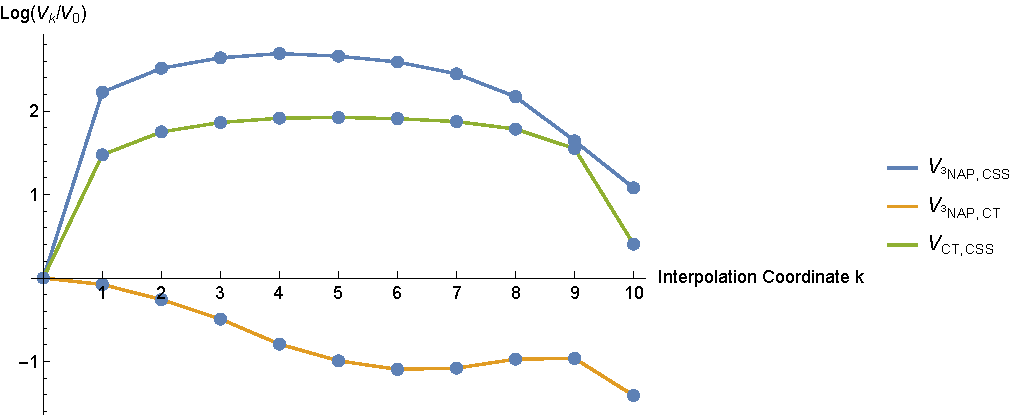
\includegraphics[width=\columnwidth]{Chapters/chap4/Images/interpolation.pdf}
\caption{Diabatic coupling values along the interpolation from the \textsuperscript{3}NAP $\rightarrow$ CT geometries. State 0 and 10 stand for the \textsuperscript{3}NAP and the CT state, respectively.\label{interCondon}}
\end{figure*}

There is another example to illustrate that the average coupling is a better value to use than the coupling at \textsuperscript{3}NAP geometry. As we have both \textsuperscript{3}NAP and CT states optimized, we can compute the energy gap between them. It is 0.81 $eV$, and is considered to be the best theoretical estimate we can get. We can also use the information at certain geometry to estimate the gap, with parabolic assumption assumed. Certainly how good the estimation is affects the computation of rate constant. Calculating at the CT state gives 0.78 $eV$, while at the \textsuperscript{3}NAP geometry gives 0.91 $eV$. If we still calculate at the \textsuperscript{3}NAP geometry, but use the average diabatic coupling, the energy gap computed decreases to 0.85 $eV$, which is much closer to 0.81 $eV$. This explains the improvement we get at \textsuperscript{3}NAP geometry by averaging diabatic coupling.

However, the results at CT geometry get worse, especially for Marcus theory. For the CT $\rightarrow$  CSS reaction, the average diabatic coupling is so unreasonable that Eq. \ref{mixingangle} does not have any real solution for $\theta$, so it is absent in Fig. \ref{rateComp}. Looking at Fig. \ref{interCondon}, we suspect that the best choice of diabatic coupling is where Condon approximation holds, i.e., where the change of coupling is slow. The proposition can be tested when the calculations of other two molecules, PTZ-CH\textsubscript{2}-Pt-NAP and OMe-PTZ-Pt-NAP are complete.


\section{Conclusion} % (fold)
% \label{sec:conclusion}
We present here a modified version of our previous approach \cite{yang2014intramolecular,yang2015computing}. We change the ER diabatization to the GMH approach and apply the model to a much more complex system. Certain success is achieved. Our approach gives reasonable rate constants and always performs better than Marcus theory, which illustrates the robustness of our model.

Weinstein's experiment demonstrates the promising future of IR-controlled electron transfer, which has huge potential in application. The theoretical study is important to understand and predict such property. The results presented here are a blend of success and failure. The calculations based on the CT state give good agreement to experiments, both in rate constant and primary mode. While \textsuperscript{3}NAP geometry gives much poorer results, but they can be partially corrected by adjusting the diabatic coupling. The cause of failure and success of our method needs more research. The undergoing calculations of other molecules can bring new tests to our method.
% section conclusion (end)



